\chapter{Testing and data analysis}\label{sec:TestingAndDataAnalysis}
This chapter goal is to show application testing, data collection and analysis.

\section{Testing environment}\label{sec:TestingEnvironment}
Test site of this application is a third floor of the Campus building of the Faculty of Informatics and Management, University of Hradec Kralove (FIM UHK). The main walk-through corridors are in a rectangular arrangement. Classrooms and offices are situated inwards and outwards in relation to the corridors. There is a roofed atrium in the center of the building. Experiments have been conducted in a 52 m x 43 m area.

\begin{figure}[H]
	\begin{centering}
		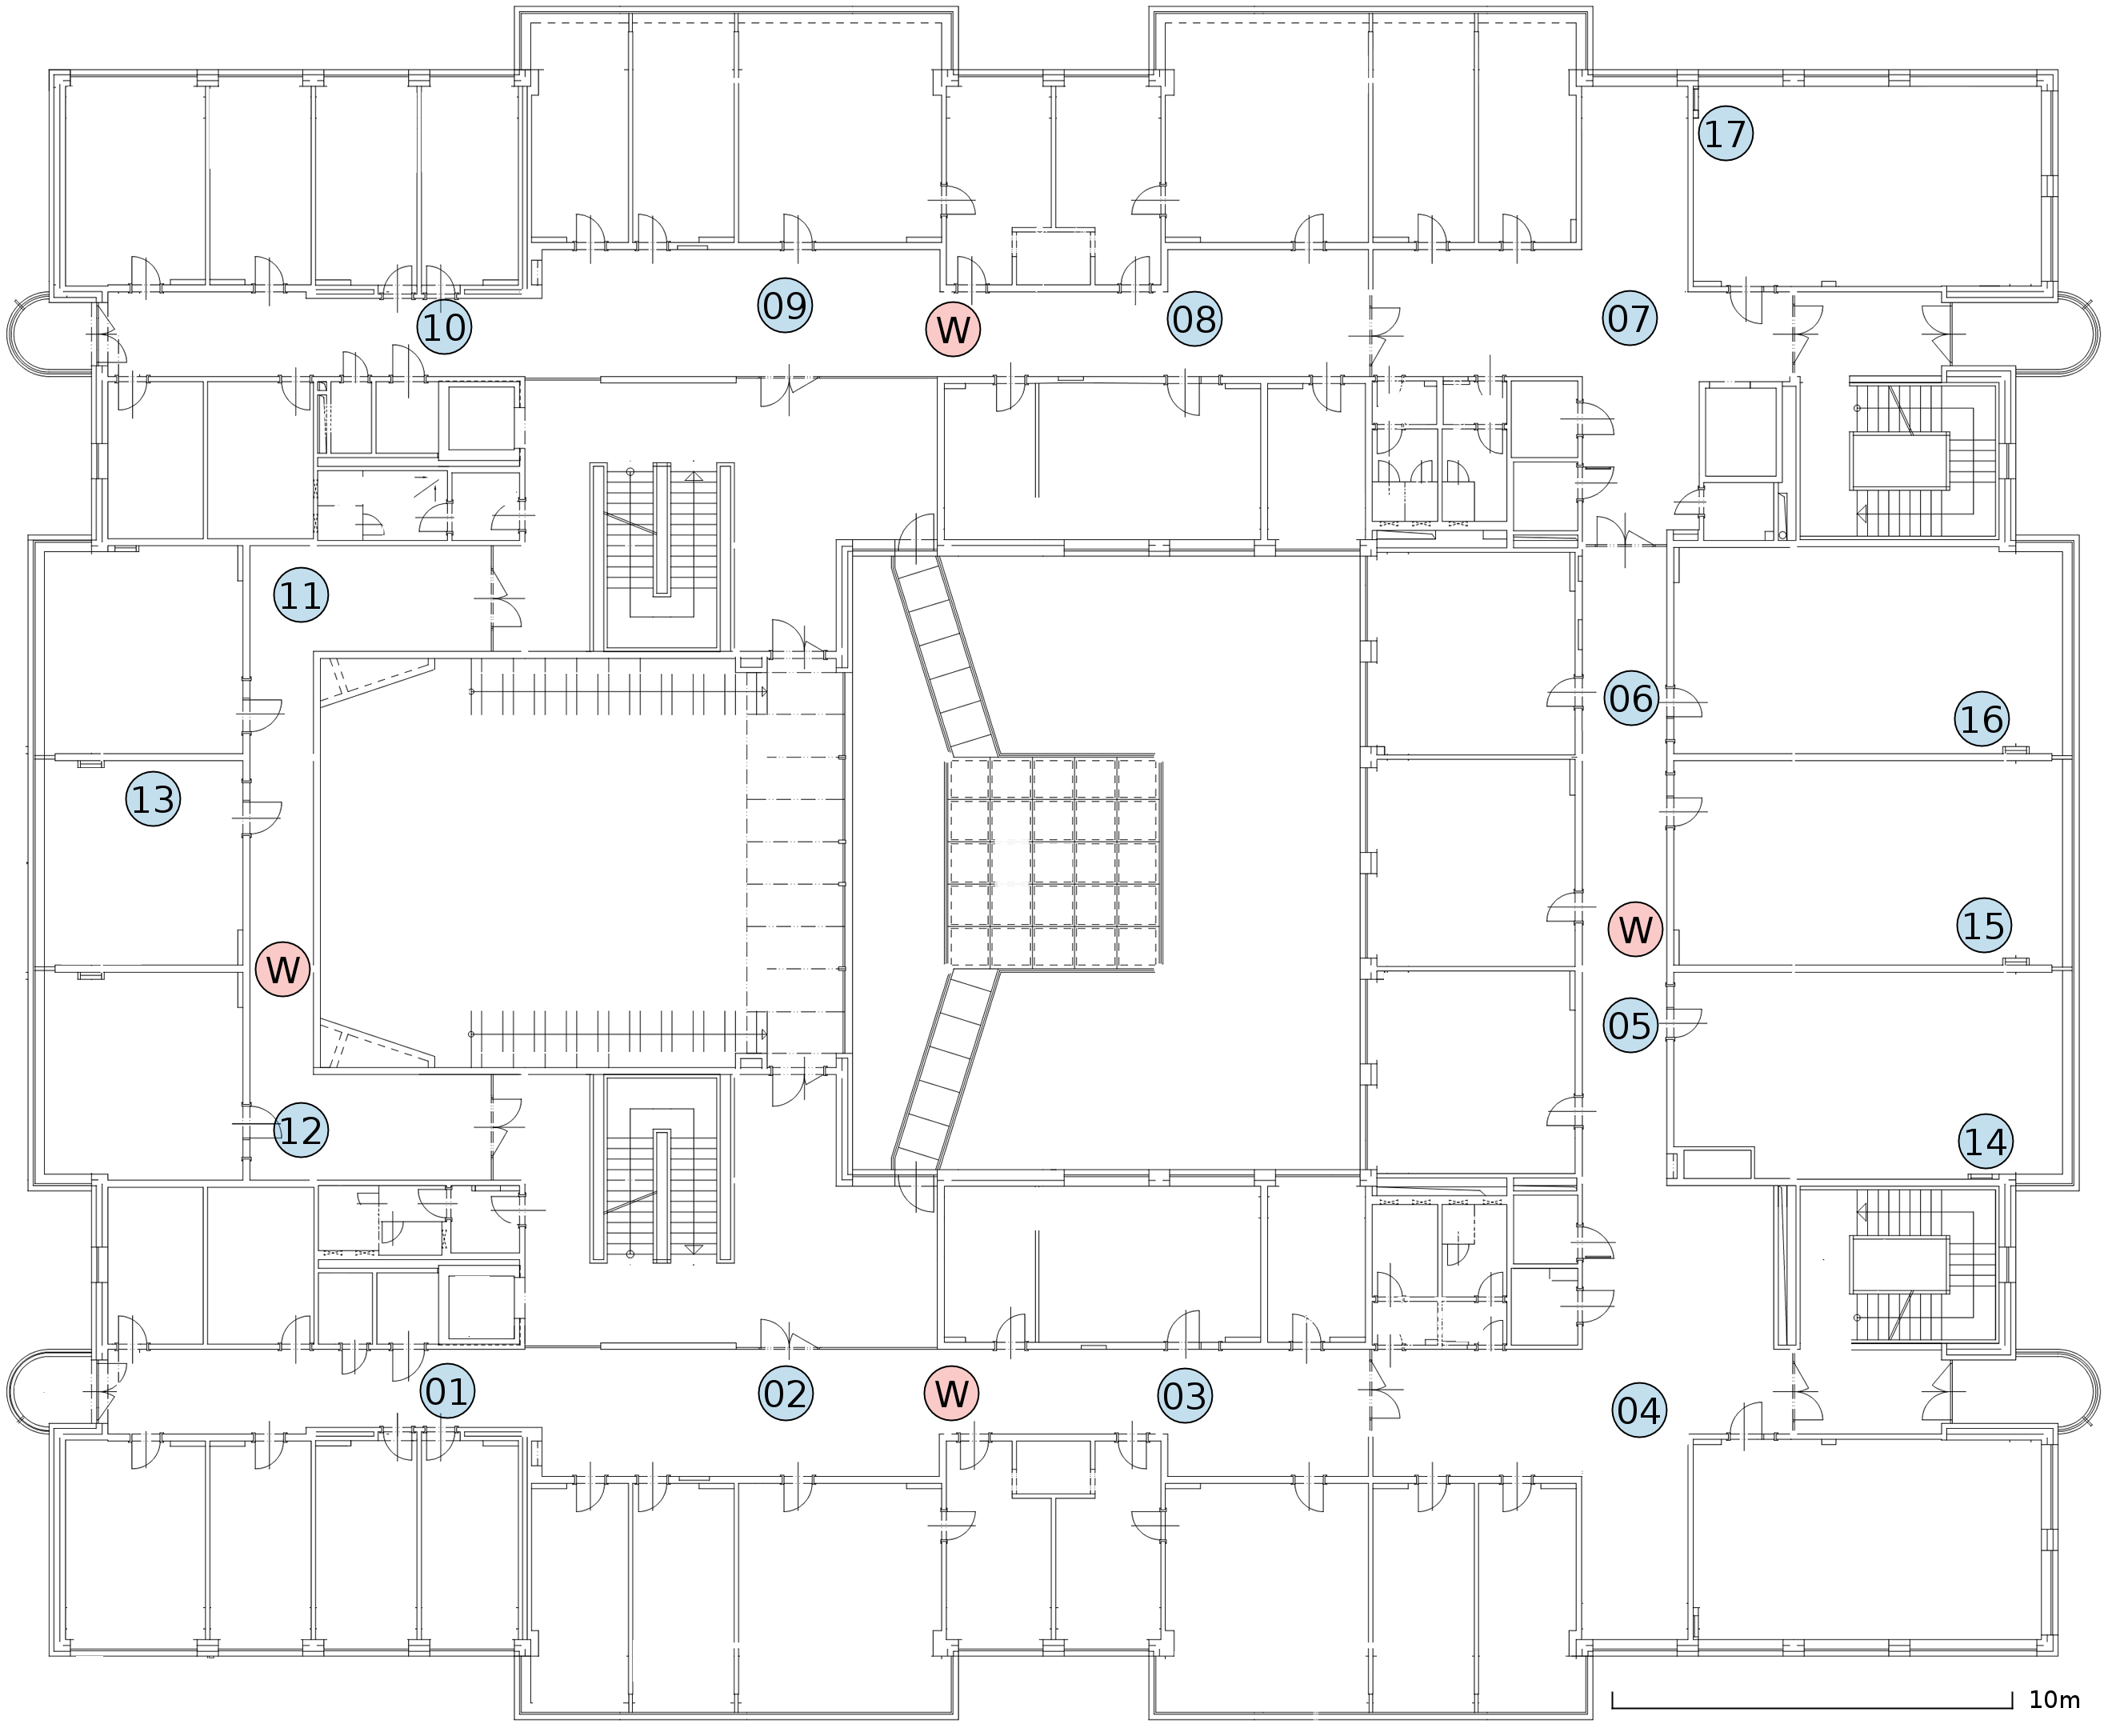
\includegraphics[width=0.8\textwidth]{img/j3np}
		\par\end{centering}
	\caption{Map of deployed devices (based on \cite{IILUBLEB})}
	\label{fig01c06}
\end{figure}

\fref{fig01c06} shows positions of deployed devices. There are four WiFi transmitters for \verb|eduroam| network made by Cisco (marked as W) on this floor. They are permanently placed on the ceiling and their settings could not be altered. Each marked place has usually more than one of them, typically at least two. One of them broadcasting in a 2.4 GHz and the other in a 5 GHz band. Their TX and power is automatically adjusted to help mitigate interference and signal coverage problems.

The other devices marked by numbers from 1 to 17 are Bluetooth Low Energy beacons placed evenly in the corridors and on the floor. They broadcast parameters were set to the advertising interval of 100 ms and the TX power of 0 dBm. Corridor beacons are placed in positions about 10 m apart from others \cite{IILUBLEB}. Since the beacons were placed two years ago there was a possibility of battery depletion and malfunction. By multiple tests we figured that two beacons had their battery depleted (1, 4), one was reconfigured and one was missing completely (5).

\section{Evaluation approach}\label{sec:EvaluationApproach}
Basics of evaluation are same as in previous year using solution created by Pavel Kriz in \cite{IILUBLEB}. This approach is using WKNN algorithm to compare fingerprints against each other by selecting one and comparing it to all other fingerprints. Basic premise of this evaluation is to pick one fingerprint, forget its position and try to calculate it via specific amount of neighbors. This calculated value is then compared to real one and difference between these values is the error in meters. Advantage of this approach is that it can be done in only one phase instead of two, since online phase is supplemented by one selected fingerprint. Second advantage is easy implementation and calculation of error difference since both calculated and real positions are known.

This evaluation it implemented to used on one fingerprint and compare it to others, implementing testing of BLE and WiFi signals separate or together it can provide an insight on which technology is better and if combining them improves the precision. This evaluation program also enables filtering out data not used for analysis, which are records of devices other than mentioned BLE beacons and WiFi access-points. Since this approach does not differentiate between technologies of recording devices it had to be expanded to support this.

\begin{itemize}
	\item Filtering data by the device type, which is an important part to enable test only for a specific device type. These fingerprints are tested only against its own technology and results can be used to compare precisions between technologies.
	\item Selecting fingerprint group, in this case multiple fingerprints are picked an tested. This selection is done via scan id, meaning both scan originated at the same time and place on different devices. Both fingerprints are tested individually but the results are combined together aiming to improve total localization accuracy. This approach enables two testing types, run the test against its own technology or all fingerprints.
	\item Combine data from multiple device technologies and consider it as one. Fingerprints are selected based on their scan id and all scanned data are cloned into mobile fingerprint combining them together.
\end{itemize}

All of these different approaches will enable to compare technologies and also show which approach has the lowest error so it could be used in the future. 

\subsection{WKNN}\label{sec:WKNN}
This approach is extends algorithm \textbf{K Nearest Neighbors} (KNN) with \textbf{Weights} making it WKNN. KNN is based on the idea that unclassified individual should belong to the same class as its nearest neighbor in the data set \cite{HGAfC}. It calculates the position based on the locations of selected K nearest neighbors, where K change influences the accuracy of this algorithm. Extended with weights, WKNN can make some neighbors or data more valuable than other ones. In this case, closer fingerprints have higher weight and will be used to calculate position by Euclidean distance formula. The equation for a fingerprint $f = (f_1,f_2,...,f_n)$ from the $i$th fingerprint $S_i = (s_{i1} ,s_{i2},...,s_{in})$ can be expressed by following formula \cite{IILUBLEB, HGAfC}:

$$D_i = \sqrt{\strut\sum_{j=1}^{N}(f_j-f_{ij})^2}\ ,$$

where N is a number of unique transmitters in the measurement.

These distance values are sorted and based on them first $k$ fingerprints are chosen to calculate weighted estimate of position $P$ of measured fingerprint. We can achieve this by using their known positions $P_i[x_i,y_i]$ in a following formula:

$$ P = 
\frac
	{\strut\sum_{i=1}^{k} P_i Q_i}
	{\strut\sum_{i=1}^{k} Q_i},\
where\
	Q_i = \frac{\strut 1}{\strut D_i}.$$

WKNN algorithm was chosen because it is easy to implement and result data are not difficult to interpret.

\section{Data collection}\label{sec:DataCollection}
Data was collected at 105 evenly-spaced (2m) positions of Campus building floor. Each position was measured four times, in two different headings (north, south) and with two device orientations, to prevent signal obstruction. Using both devices, 105 positions and 4 scans per position resulted in 840 different measurements consisting of 466 411 BLE and 73 757 WiFi individual RSSI samples making it in total 540 168.

Each of the scans was run for 30 seconds on both devices at the same time to provide equal environment. It is not really feasible to run such long scans in one run, so the decision was made to split sub-scans into smaller time intervals. BLE beacons have advertising interval set to 100 ms and single scan length could be set to this number but it is set to 200 ms to prevent packet loss between the scans. Since localization using WiFi usually does not need big amount of data, scanner is set to run every 5 seconds. One problem with this scanner is that Android does not allow to set scan length or cancel WiFi scanning, only thing that can be canceled is listening for new WiFi records but scan could still be running. The result of this may be that current scan receives data from previous one, this is not prevented in the application but it can be filtered out for evaluation. Cellular and sensor scanner are set to same length as WiFi since this data is used only as complimentary and it helps to reduce fingerprint data size.

Three data collection sessions were run during application development and data from the last one were used for evaluation. To consider fingerprint viable it must contain at least 20 records for Bluetooth Low Energy and WiFi, otherwise it needs to be deleted and re-scanned.

\subsection{First data collection}\label{sec:FirstDataCollection}
This first collection was meant as a test run in real environment and it consisted of scanning ten spots, each was scanned three times for 20 seconds to check if the scanner is reliable. This session revealed two main problems with the scanner.

First, with WiFi scanning on wear device where the scanner did not find any data. It was probable that there was a problem with scan length since quick 30 seconds test showed data added at the last second. This was fixed by two main changes, increasing scan length to 30 seconds and more importantly wear device now starts a WiFi scan right after the activity is displayed and before actual scanning is triggered. These changes helped to improve this scanner and it does not create any problems since there is little time between this \enquote{dummy} scan and the actual scan, usual time difference is in milliseconds.

Second, not enough data was received by BLE scanner. Data from previous years showed that each scan usually has hundreds of BLE records but this scanner was able to collect around 50 of them. It was later discovered that scan times were not properly set for AltBeacon library and scanner was run for 1 second instead of 200 milliseconds with only one device record per scan.

After both of these issues were fixed it second data collection was run to collect the data for evaluation. And there is one final thing to note, which is that wear device was not able to scan any Cellular records even though specification shows it should support LTE technology. 

\subsection{Second data collection}\label{sec:SecondDataCollection}
This collection was meant to be the final one and the data should have been used for evaluation, but there were problems revealed all the data was collected. All data seemed fine but evaluation showed problems with BLE beacons. For a start, analysis data informed that around 30 fingerprints were removed from testing due to no specific BLE beacons found. Most of these fingerprints originated on wear device.

\begin{table}[h]
	\begin{center}
		\begin{tabular}{ l C{2cm} C{2cm} C{2cm} }
			\hline
			Max error (m) & BLE & WiFi & Combined \\ 
			\hline
			All devices & 27 & 14 & 11 \\ 
			Mobile & 30 & 14 & 11 \\ 
			Wear & 31 & 11 & 11 \\ 
			\hline
		\end{tabular}
		\caption{Maximum errors for second data collection}
		\label{tab01c06}
	\end{center}
\end{table} 

\tref{tab01c06} shows a table of maximum errors in meters for collected data, as it shows BLE errors can be two or three times higher then of WiFi ones reaching almost 30 meters error which would place the device on the other side of the building. Mean and median errors showed the same trend so next step was to test if some beacons are missing in the data and display errors on the map to find the worst locations.

\begin{figure}[H]
	\begin{centering}
		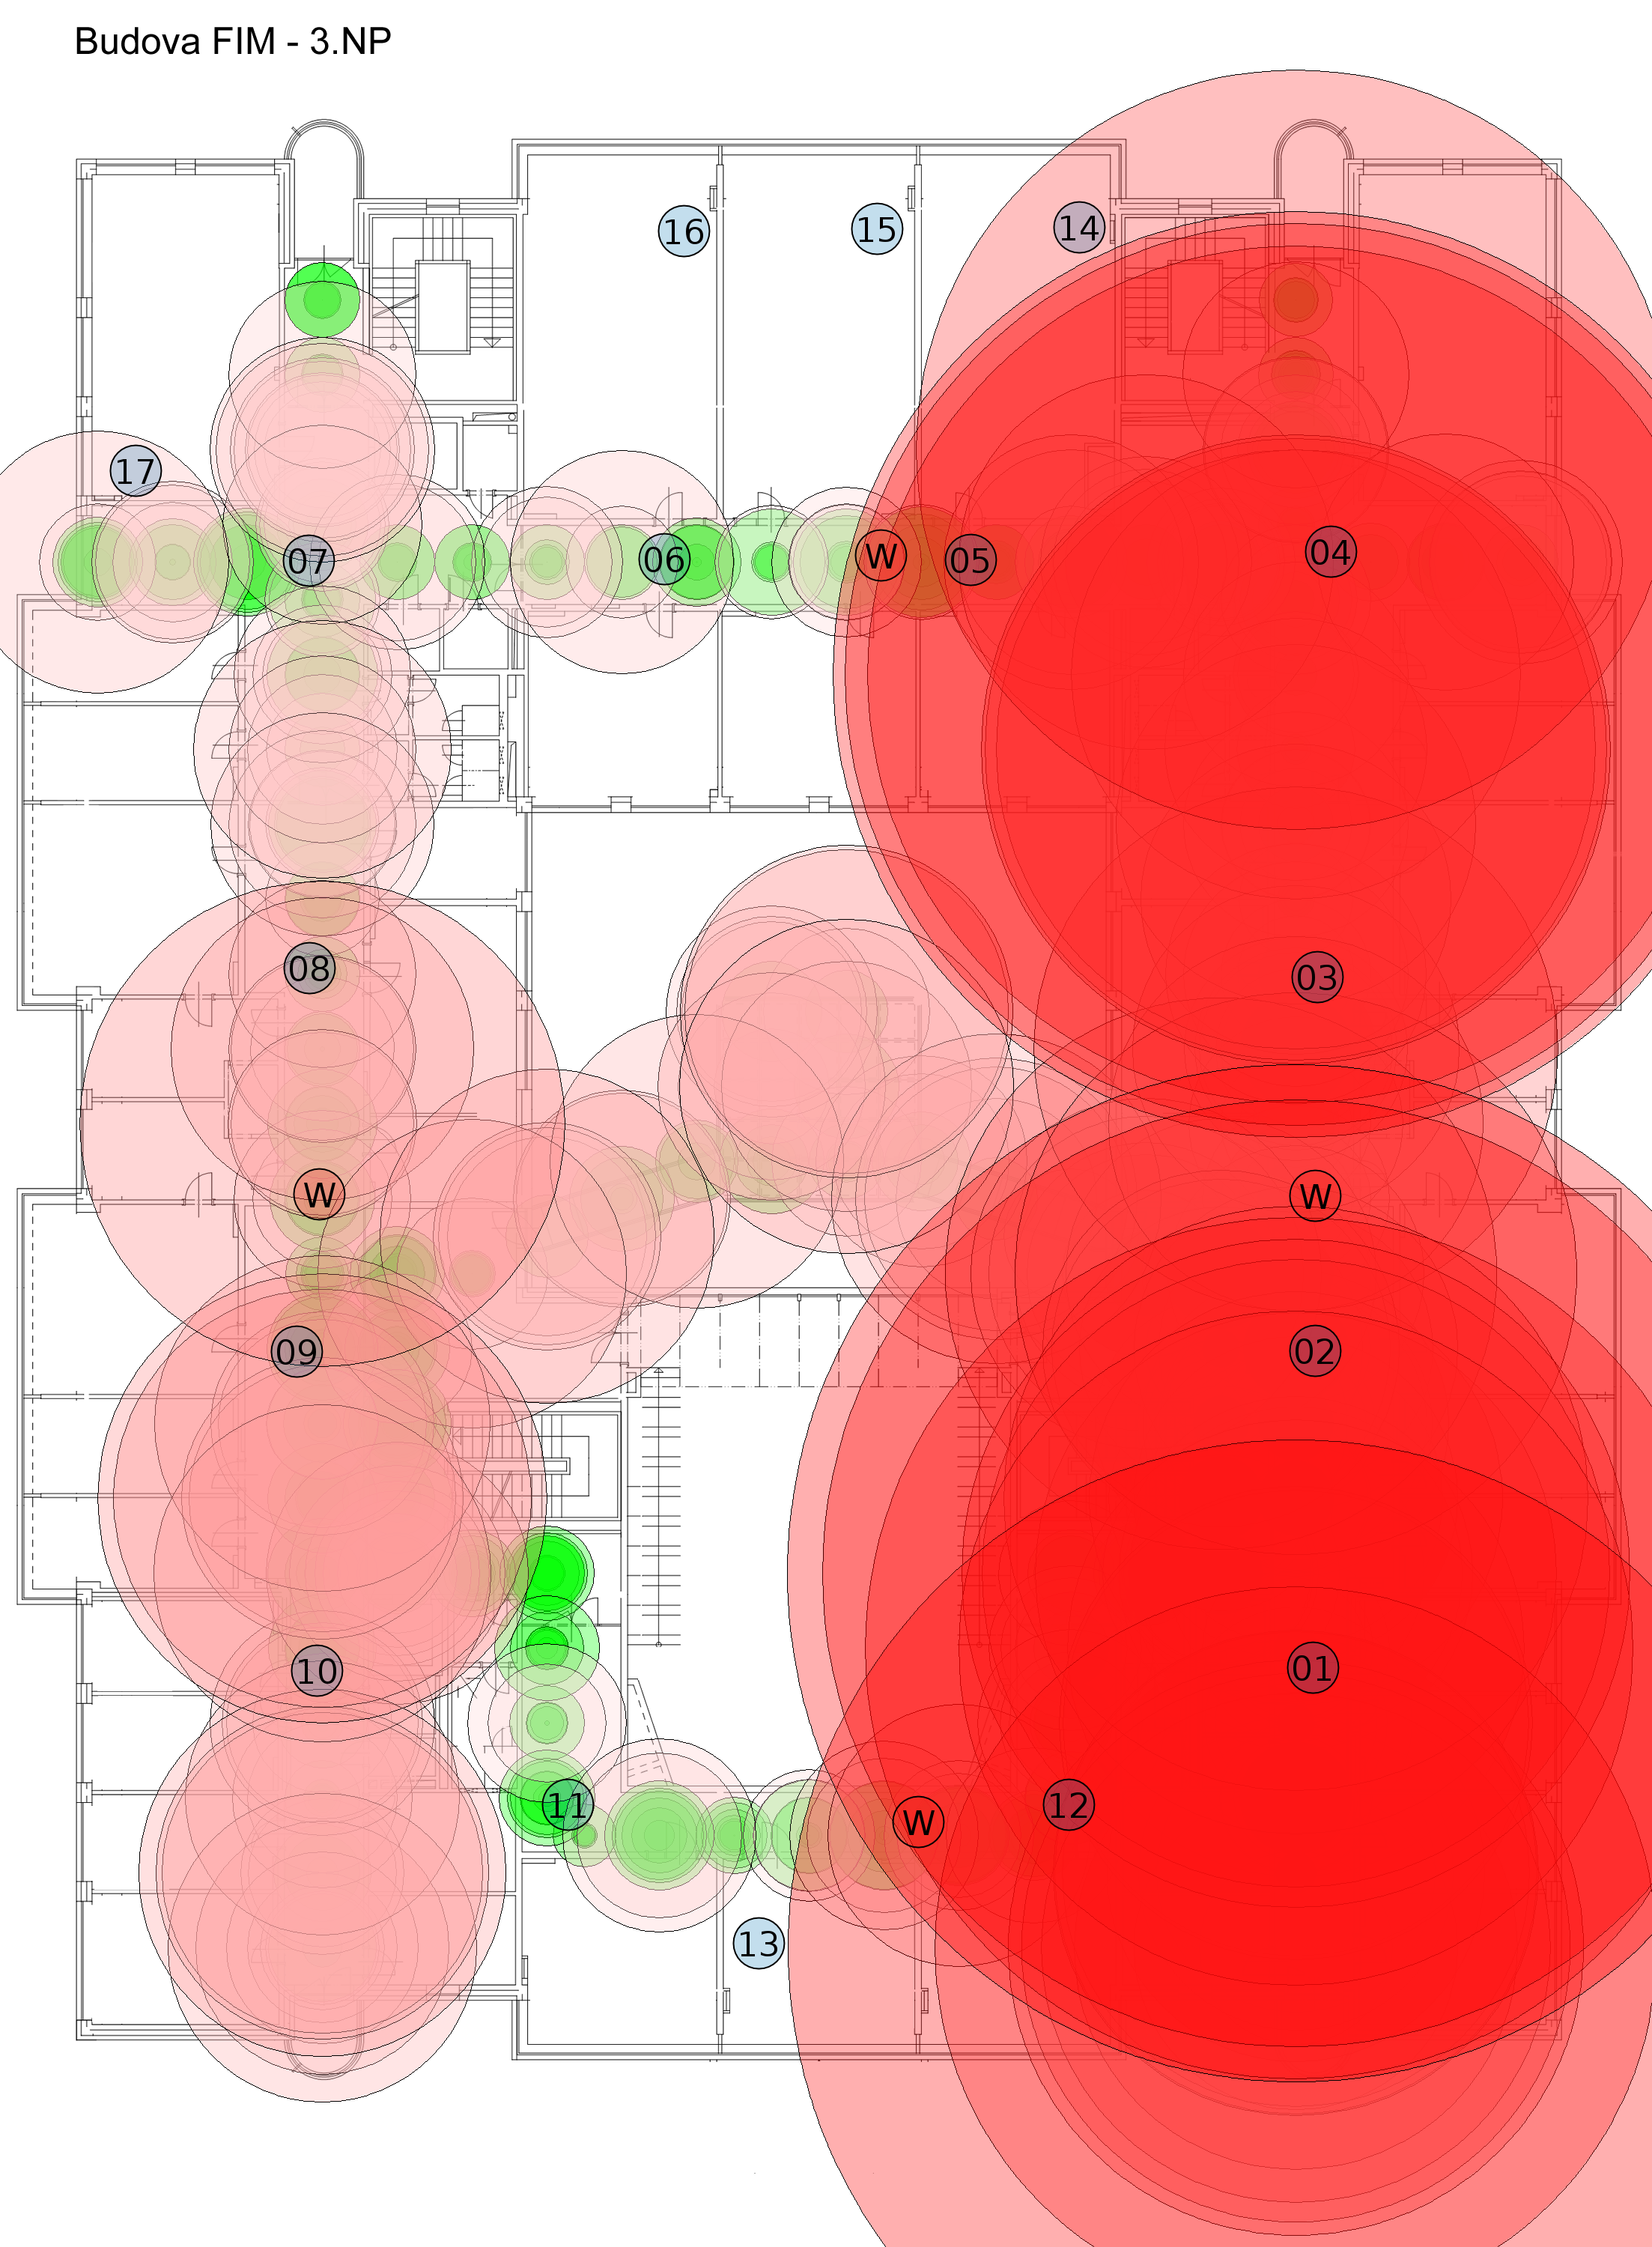
\includegraphics[width=0.5\textwidth]{img/second_data_collection_errors}
		\par\end{centering}
	\caption{Map of errors for BLE in meters for all fingerprints}
	\label{fig02c06}
\end{figure}

\fref{fig02c06} shows errors on BLE scanning on the map with two indications of error size. First, circle size is calculated from error number, the higher error = bigger the circle. Second, fingerprints with error under three meter have green color and those above have color based on their error in red spectrum, more saturated red = higher error. Judging based on these information evaluation seems to be worst near beacons 1 and 4, which were later found out to be out of power. Next evaluation using differences in advertising interval revealed beacon number 14 reconfigured to different settings. Final tests were to check if all beacons are in place where number 5 was moved and had to be replaced. All of these tests resulted in four malfunctioning beacons all over the floor and deeming the data not viable to further evaluation, hence new data collection was required.

Since this was a complete data collection it also served as a test for wear device how long it can stay operational and scanning. Multiple data were collected to measure this, such as start and end time, number of places and fingerprints scanned and of course power status. Wear device is never used under 15\% because this is the threshold when power saving is turned on and device shuts down all non essential functions.

\begin{table}[h]
	\begin{center}
		\begin{tabular}{ l C{2cm} C{2cm} C{2cm} C{2cm} }
			\cline{2-3}
			& \multicolumn{2}{c}{\% Battery power} & & \\
			\hline
			Time & Start & End & Places & Fingerprints \\ 
			\hline			
			2:50 & 100\% & 15\% & 30 & 240 \\
			2:40 & 100\% & 17\% & 37 & 296 \\
			1:55 & 100\% & 35\% & 12 & 96 \\
			1:20 & 100\% & 70\% & 18 & 144 \\
			0:45 & 30\%	& 15\% & 8 & 64 \\
			\hline
		\end{tabular}
		\caption{Scanning information for wear (second scan)}
		\label{tab02c06}
	\end{center}
\end{table}

\tref{tab02c06} shows all important information for wear scanning. First thing to note when comparing the percentages of power with time is that wear device cannot usually last for more than three hours of scanning, which is no enough since all the scans took about 8 hours to complete. First two long scans show that wear can scan for around 35 places without the need for charging, which is confirmed by short scan where scanning 8 places takes around 45 minutes and 15\% of the device battery. There are also some exceptions like the third scan which was done in the middle of Campus building where there are now beacons and it was needed to re-scan multiple places many times to achieve set requirements mentioned in previous chapter.

\subsection{Third data collection}\label{sec:ThirdDataCollection}
Third and final data collection was conducted after all beacons were checked and fixed. Scanning showed only one single problem and that is again with the WiFi scanning on wear where no records are found usually after 10 spots, 80 fingerprints, were collected. This is not a huge issue that has two easy fixes. First, is restarting the device which will enable to scan for 10 more spots without problems. Second and not ideal is to turn off and on the WiFi receiver on the wear device. This fix only works for next two or three scans so it is not ideal. Both of these solutions were used based on the situation but wear was always turned on and off after 15 successful spots.

\begin{table}[h]
	\begin{center}
		\begin{tabular}{ l C{2cm} C{2cm} C{2cm} C{2cm} }
			\cline{2-3}
			& \multicolumn{2}{c}{\% Battery power} & & \\
			\hline
			Time & Start & End & Places & Fingerprints \\ 
			\hline			
			2:40 & 100\% & 15\% & 37 & 296 \\
			2:00 & 100\% & 33\% & 30 & 240 \\
			1:10 & 100\% & 58\% & 18 & 144 \\
			0:45 & 50\% & 22\% & 11 & 88 \\
			0:40 & 40\% & 15\% & 9 & 72 \\
			\hline
		\end{tabular}
		\caption{Scanning information for wear (third scan)}
		\label{tab03c06}
	\end{center}
\end{table}

For this scan only one specific change was made and that was starting \enquote{dummy} scan also for a mobile device, before this collection it was implemented only on wear device. It was changed to provide even more equal environment for both devices and make scanning procedure completely the same. Collecting of all fingerprints took about 7 hours and 15 minutes which is almost an hour less then previous which took 8 hours and 10 minutes. Battery information in \tref{tab03c06} confirm results from previous scans and show that wear device cannot scan more then three hours at the time before reaching power saving mode. This feature can be disabled after new update of wear device system but it was not used anyway since there is no guarantee it will disable all parts of power saving.

\begin{figure}[h!]
	\begin{centering}
		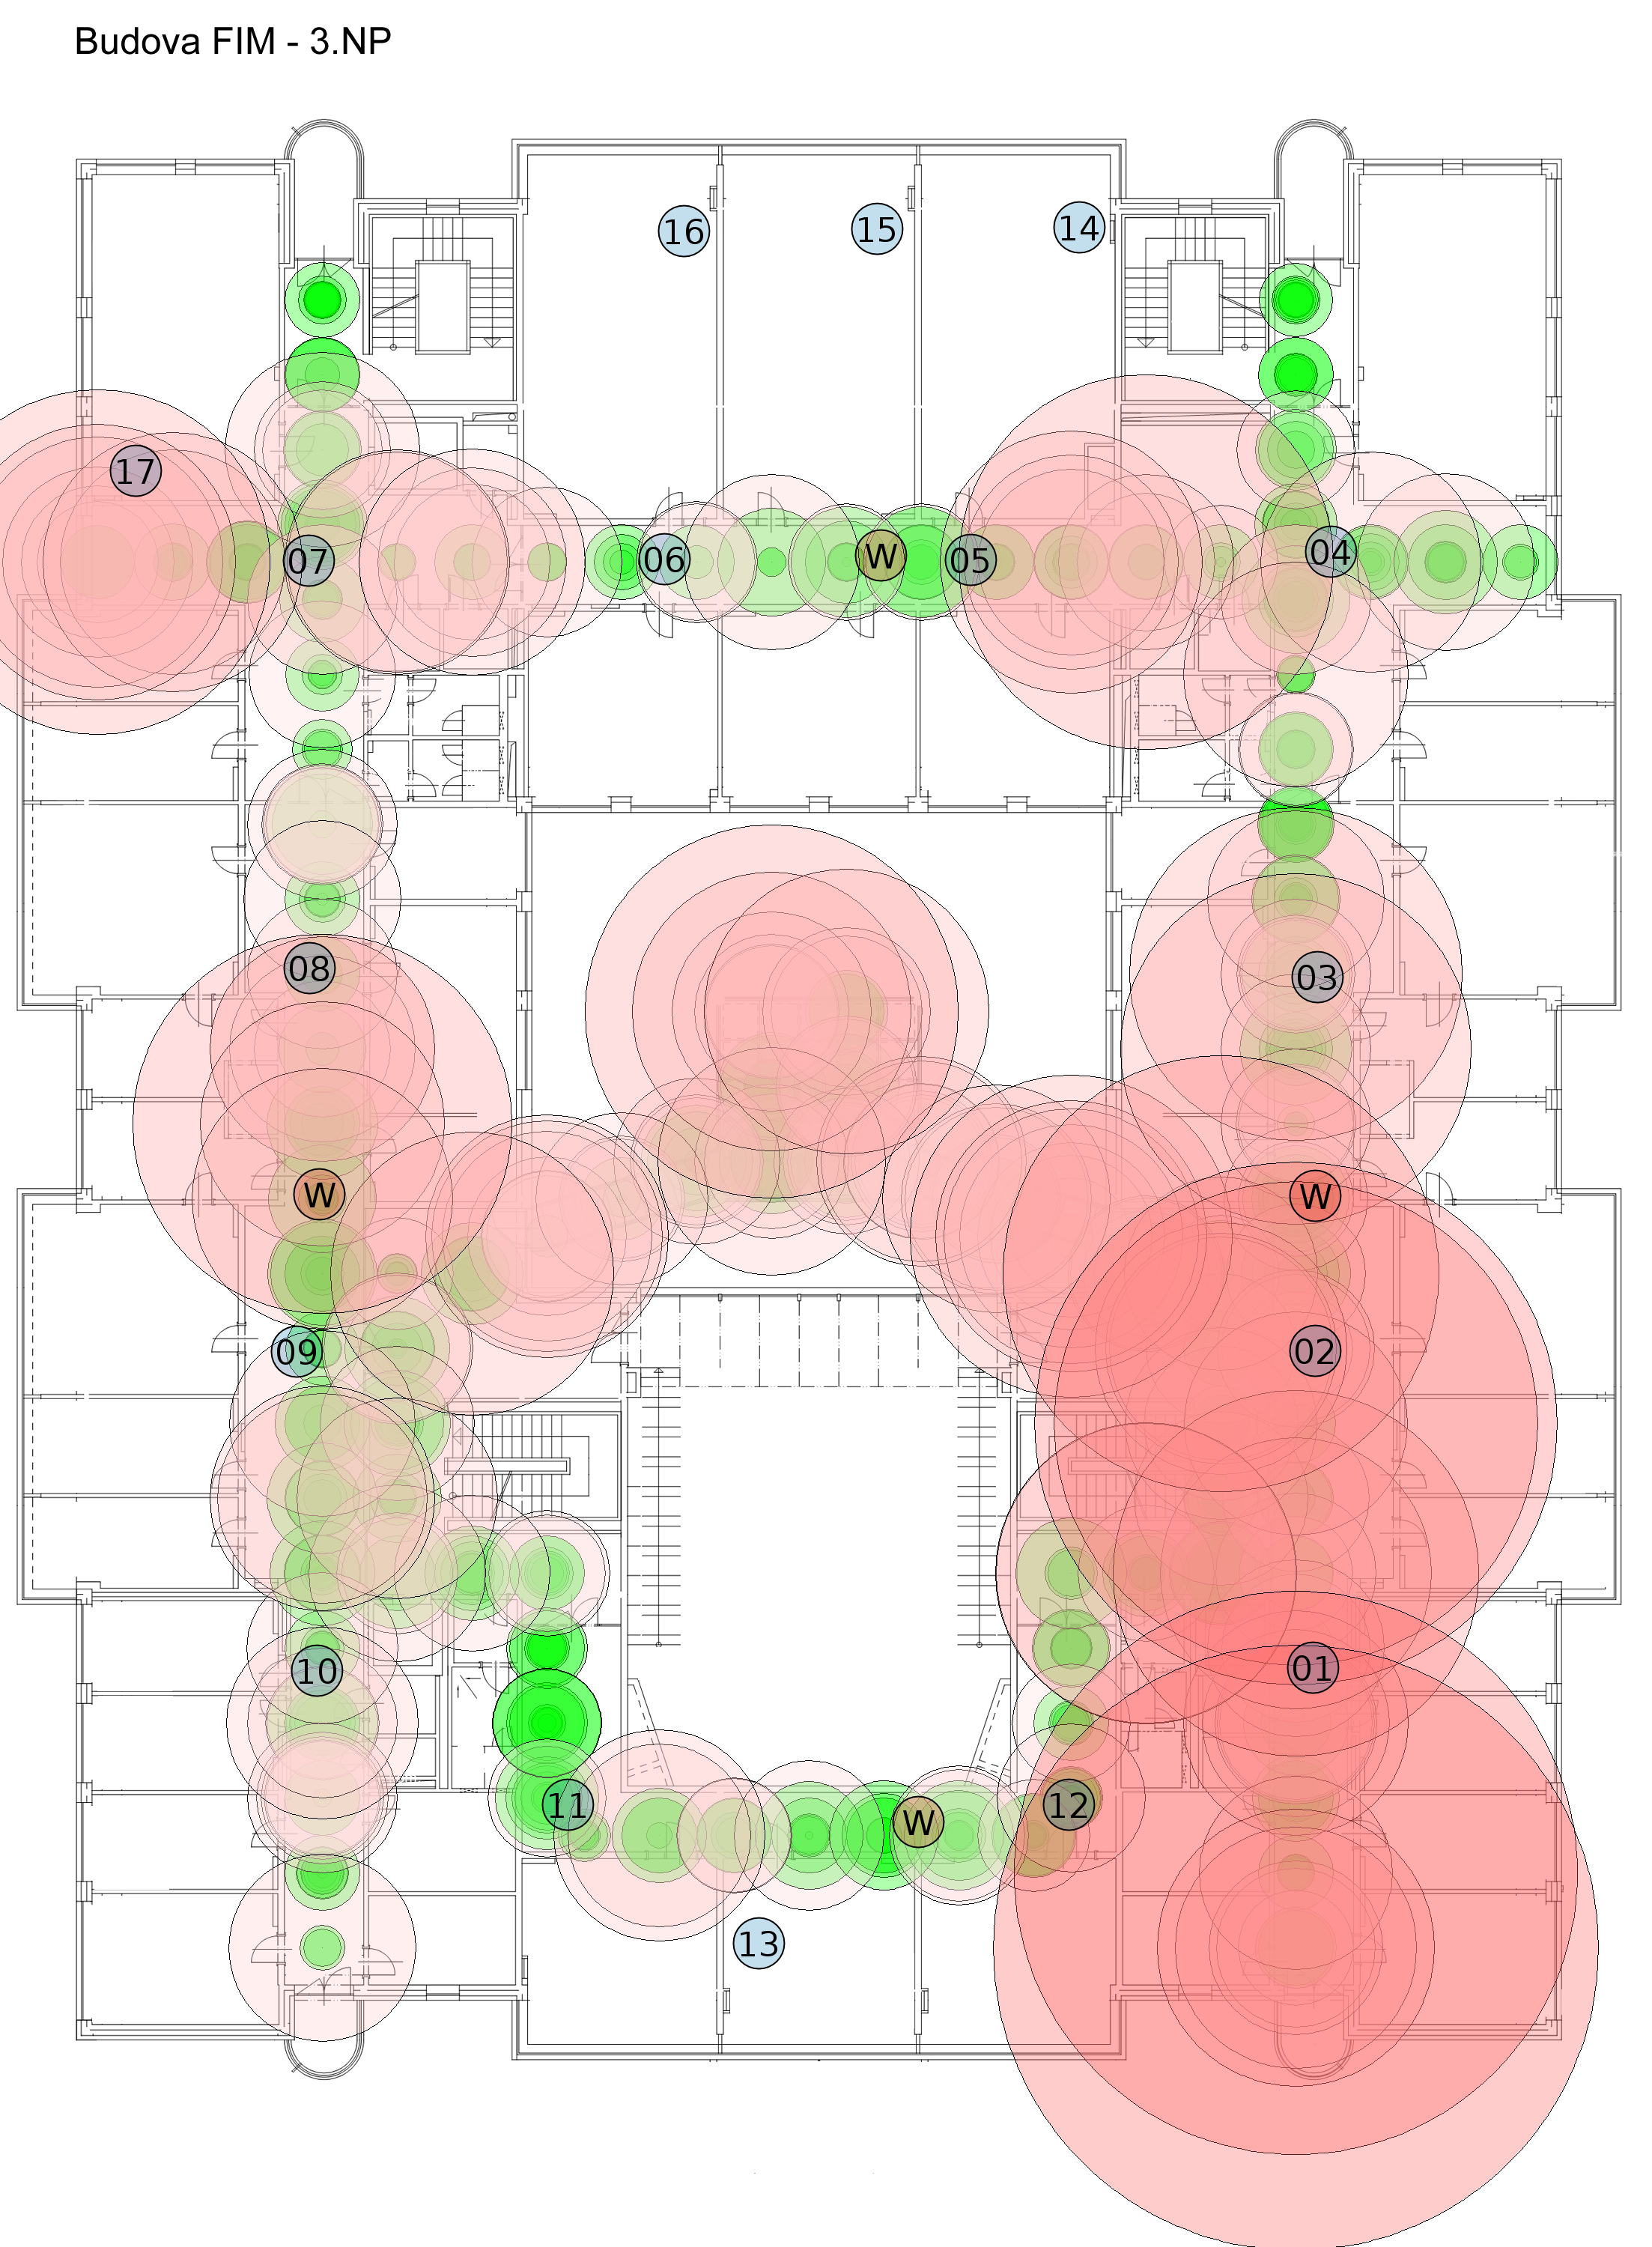
\includegraphics[width=0.4\textwidth]{img/third_data_collection_ble_errors}
		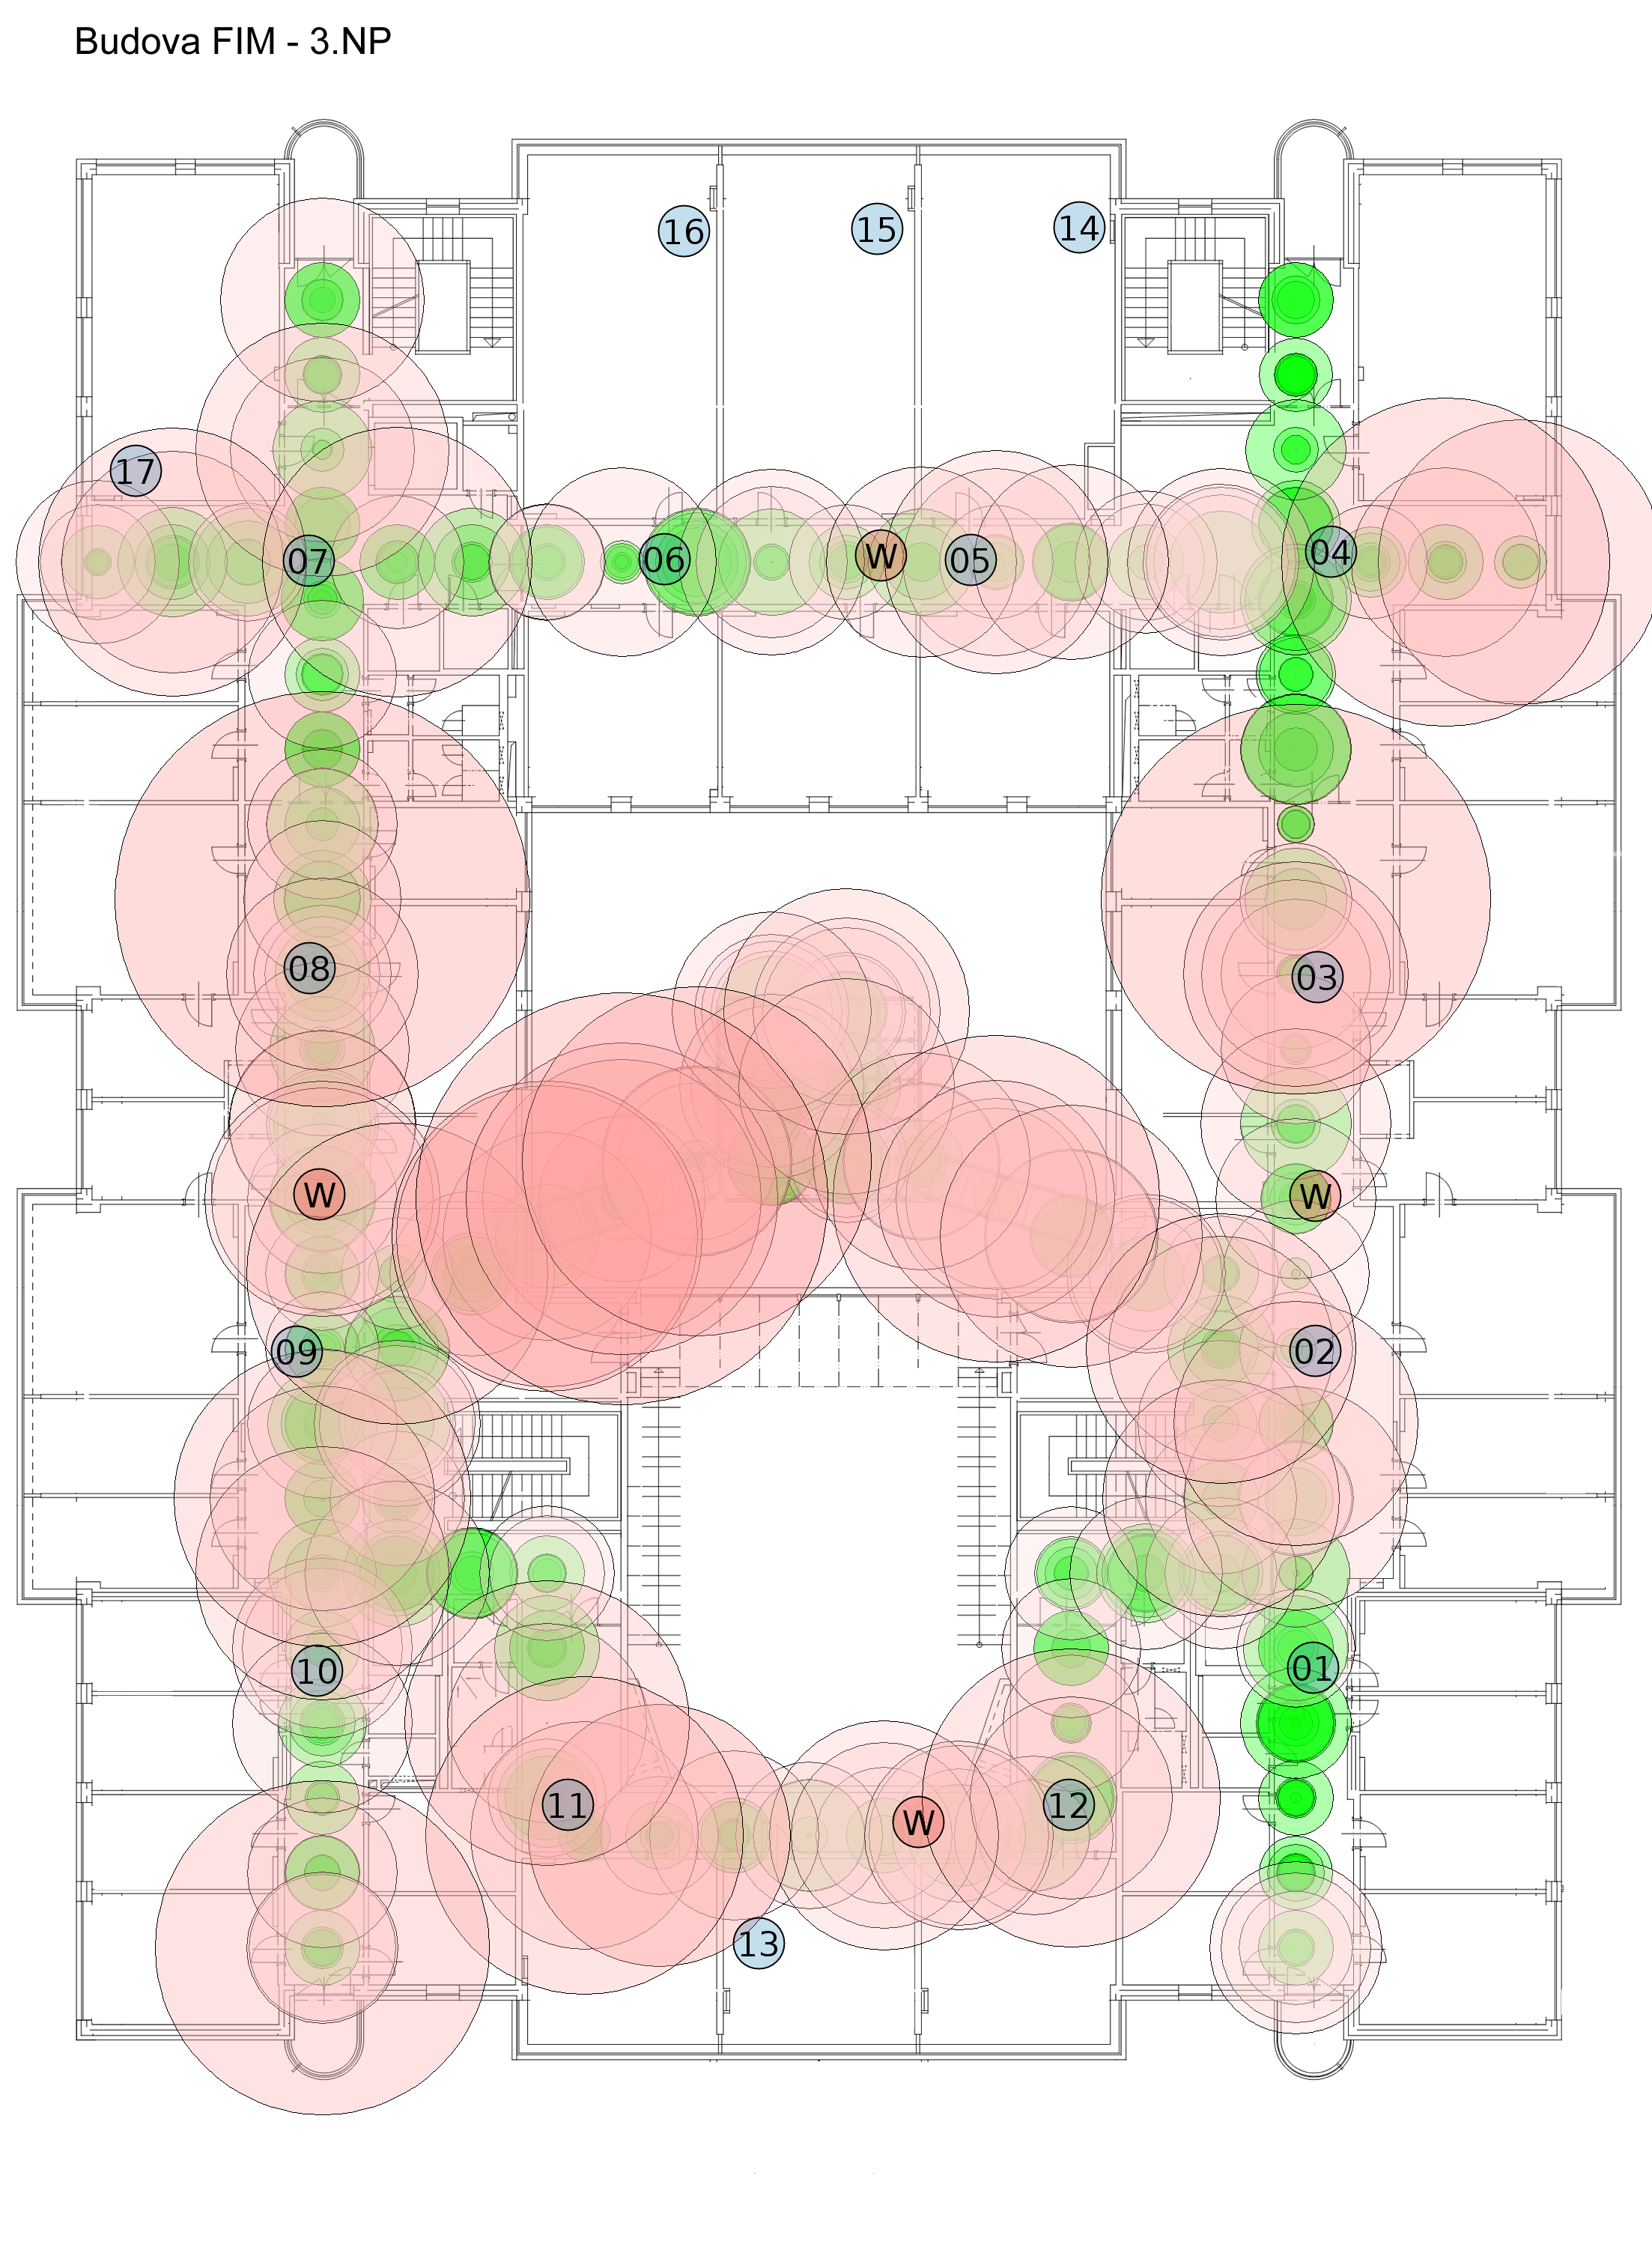
\includegraphics[width=0.4\textwidth]{img/third_data_collection_wifi_errors}
		\par\end{centering}
	\caption{Map of errors for BLE (left) and WiFi (right)}
	\label{fig03c06}
\end{figure}

\fref{fig02c06} shows two images of all fingerprint errors on the map thus creating eight overlapping circles on each spot. WiFi seems more precise in comparison with BLE and there might still be some problems around beacon 1. Places with one or two light red circles will usually be improved by other fingerprint on that spot but the others could increase localization error. On the other hand comparison of this figure and \fref{fig01c06} shows decrease of BLE errors for this scanning round. Comparison between WiFi and BLE suggests that WiFi should have smaller error and better accuracy but there might be issues for both technologies in the middle of the building.

\section{Evaluation}\label{sec:Evaluation}
Evaluating of all the data has multiple approaches and combinations since in needs to consider information such as algorithm implemented or multiple device types and radio signal technologies. During data collection was figured out that wear device is not able to scan for Cellular records so this radio signals will not be tested in the evaluation. First thing that needs to be decided is which $k$ variable to use with evaluations using WKNN algorithm and after that multiple tests can be run to compare device types and how data can be used to improve each other.

\subsection{Decide K values for WKNN}\label{sec:TestingKValuesForWKNN}
For selecting $k$ value all data was tested without their device information, thus putting all the data together and test them against each other. Only $k \in \{2, 3, 4\}$ were used in final testing because using $k = 1$ defeats the purpose of WKNN algorithm and setting $k > 4$ results with too big errors. Following tangle shows collection of mean, median and maximum errors in meters for all tested $k$ values.

\begin{table}[h]
	\begin{center}
		\resizebox{\textwidth}{!}{
			\begin{tabular}{ l C{2cm} C{2cm} C{2cm} | C{2cm} C{2cm} C{2cm} | C{2cm} C{2cm} C{2cm} }
				\cline{2-10}
				& \multicolumn{3}{c|}{K = 2} & \multicolumn{3}{c|}{K = 3} & \multicolumn{3}{c}{K = 4} \\
				\hline
				& BLE & WiFi & Combined & BLE & WiFi & Combined & BLE & WiFi & Combined \\ 
				\hline	
				Mean & 2.25 & 1.77 & 1.52 & 2.20 & 1.76 & 1.52 & 2.15 & 1.80 & 1.56 \\
				Median & 1.93 & 1.06 & 1.02 & 1.76 & 1.30 & 1.22 & 1.61 & 1.32 & 1.06 \\
				Maximum & 12.90 & 11.11 & 10 & 12.59 & 11.38 & 9.67 & 13.28 & 10.60 & 9.39 \\
				\hline
			\end{tabular}
		}
		\caption{List of errors for multiple K values}
		\label{tab04c06}
	\end{center}
\end{table}

Mean and median information are main decision variables and maximum is used only as a complimentary information. Considering values by technology it seems $k = 2$ is best for WiFi and $k = 4$ for BLE so it will be decided between these two. Combining technologies together shows mean and median are better for $k = 2$ and maximum for $k = 4$. Main variables are better when using $k = 2$ and that is why it was selected for next evaluations. It also achieves better accuracy with WiFi, which is more precise than BLE technology, and this value was already tested and used in previous years \cite{IILUBLEB}.

\begin{figure}[h!]
	\begin{centering}
		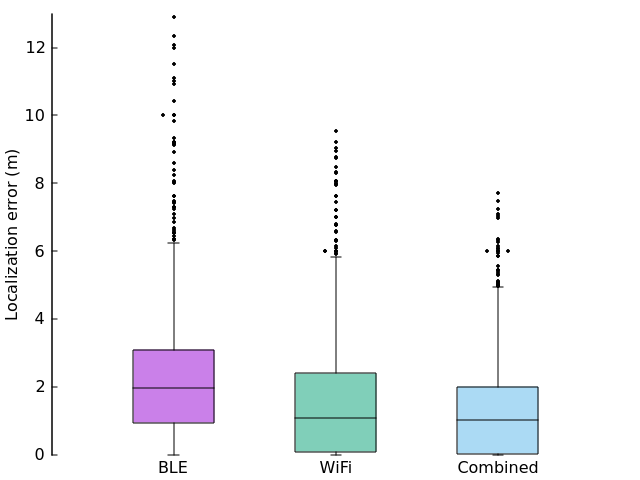
\includegraphics[width=0.5\textwidth]{img/wknn_errors_classic}
		\par\end{centering}
	\caption{Comparison of localization accuracy for $k = 2$}
	\label{fig04c06}
\end{figure}

\fref{fig04c06} shows comparison of both radio technologies used for evaluation and their combination. It correlates with \tref{tab04c06} showing WiFi better than BLE and their combination improved than using single of these technologies. This graph is mainly used to compare this evaluation method with future iteration of WKNN algorithm considering device technology recording fingerprints.  

\subsection{Compare device technologies}\label{sec:CompareDeviceTechnologies}
After it is knows which parameters to use evaluation of device technologies can be started. For this part minimum of data filtering was used and all the fingerprints were tested based on the device technology. To compare all data were also put together and tested against each other without taking device technology into consideration, meaning position of phone fingerprints can be calculated using wear fingerprints and vice versa. This is not the best approach since it defeats the purpose of using different device types but it is easily implemented for the first round of evaluation.

\begin{table}[h]
	\begin{center}
		\resizebox{\textwidth}{!}{
			\begin{tabular}{ l C{2cm} C{2cm} C{2cm} | C{2cm} C{2cm} C{2cm} | C{2cm} C{2cm} C{2cm} }
				\cline{2-10}
				& \multicolumn{3}{c|}{Mean error (m)} & \multicolumn{3}{c|}{Median error (m)} & \multicolumn{3}{c}{Max error (m)} \\
				\hline
				& BLE & WiFi & Combined & BLE & WiFi & Combined & BLE & WiFi & Combined \\ 
				\hline	
				Wear & 2.27 & 2.67 & 2.21 & 2.00 & 2.10 & 2.00 & 12.90 & 11.11 & 10 \\		
				Mobile & 2.05 & 0.88 & 0.85 & 1.76 & 0.80 & 0.88 & 11.50 & 8 & 6.06 \\
				All devices & 2.25 & 1.77 & 1.52 & 1.93 & 1.06 & 1.02 & 12.90 & 11.11 & 10 \\
				\hline
			\end{tabular}
		}
		\caption{Device comparison: mean and max errors (in meters)}
		\label{tab05c06}
	\end{center}
\end{table}

\tref{tab05c06} shows the comparison of device fingerprints and their calculated Mean and Max error values. BLE technology does not show much of a difference in devices, just in about 0.2 meters which makes them comparable. The WiFi, on the other hand, shows a big difference between these two types making mobile a better solution with over two times lower mean error. Fingerprint data were checked to find precise reason behind this difference.

\begin{figure}[h!]
	\begin{centering}
		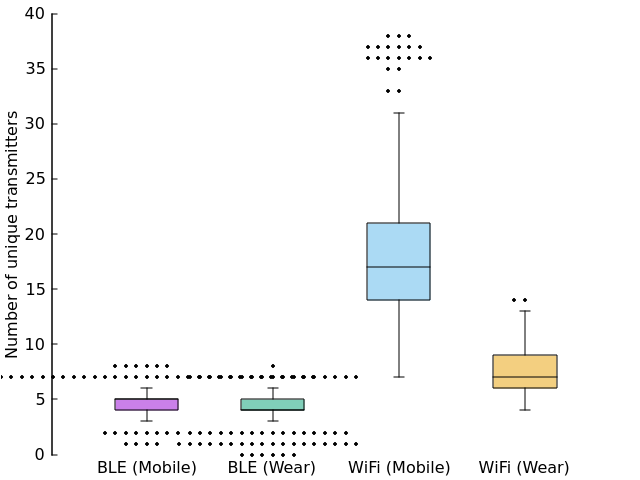
\includegraphics[width=0.6\textwidth]{img/number_of_transmitters}
		\par\end{centering}
	\caption{Number of transmitters for all fingerprints}
	\label{fig05c06}
\end{figure}

\fref{fig05c06} shows number of transmitters for all fingerprints based on technology and device. It shows close numbers for BLE but there seems to be lower amount of WiFi transmitters for wear device. It seemed that wear was not able to record signals from some transmitters and after comparing data from wear to mobile it was discovered that missing transmitters use 5 GHz technology. Mobile fingerprints contain over 7 300 WiFi records originating from access-point on 5 GHz where wear has 0 of them. Thus figuring out that wear device does not contain 5 GHz WiFi receiver. Every manufacturer is in control of hardware for its devices and Huawei decided not to implement it due to high power usage. Records from 5 GHz are more precise than those of 2.4 GHz making this a reason why wear precision is not as good when comparing to mobile device.

Combining data from both wireless technologies together and comparing devices shows wear error almost three times higher than of mobile device, thus increasing the error when combining all data together. It increases mean error from mobile only 0.85 to 1.52 combined and max from 6.06 to 10, meaning using only mobile device would result in better precision instead of combining both in this case. It is connected to already mentioned WiFi precision of wear device.

\begin{figure}[h!]
	\begin{centering}
		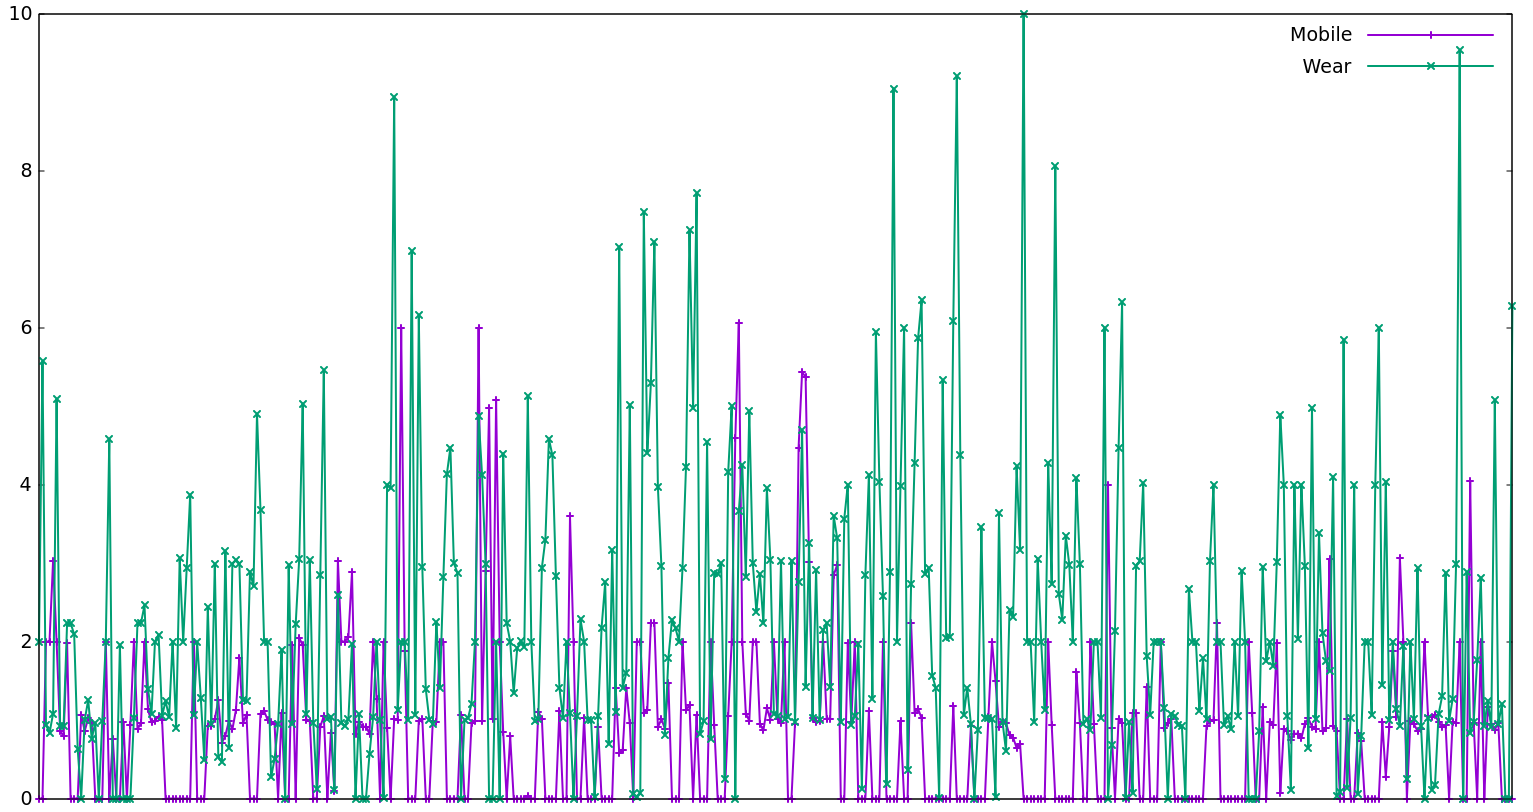
\includegraphics[width=1\textwidth]{img/wknn_errors_mobile_phone}
		\par\end{centering}
	\caption{Comparison of errors based on device}
	\label{fig06c06}
\end{figure}

To compare both technologies more precisely all fingerprint errors were sorted are displayed in \fref{fig06c06}. The image confirms information that using wear device fingerprints will result in higher error than mobile but there is few places where using wear is better, but unfortunately there is not a lot of them. 

\subsection{Testing multiple fingerprints}\label{sec:TestingMultipleFingerprint}
Previous method is testing only single fingerprint against all other ones without the device type information. Improving upon previous design this evaluation selects multiple (two in this case) fingerprints with different device origins and runs the WKNN on them. These fingerprints have to be from the same location and also from the same scan group, which is identifies by their scan id. All of these fingerprints have their location calculated and this information is then averaged to increase the location precision. This algorithm supports multiple technologies and it could be improved to support weights where specific technology, such as mobile, could have higher weight to reduce influence of technologies with worse precision.

There are two main implementation of this evaluation. First, compares both fingerprints to all ignoring device technology like previous evaluation. Second, each of the fingerprint is compared only to its own origin device type which is used to check the influence to calculations based on data sources, thus figuring out if testing fingerprints against its own technology can improve or make the precision worse.

\begin{table}[h]
	\begin{center}
		\resizebox{\textwidth}{!}{
			\begin{tabular}{ l C{2cm} C{2cm} C{2cm} | C{2cm} C{2cm} C{2cm} }
				\cline{2-7}
				& \multicolumn{3}{c|}{Compared to own technology} & \multicolumn{3}{c}{Compared to all} \\
				\hline
				& BLE & WiFi & Combined & BLE & WiFi & Combined \\ 
				\hline	
				Mean & 2.18 & 1.77 & 1.53 & 2.30 & 1.77 & 1.52 \\
				Median & 1.87 & 1.50 & 1.33 & 1.99 & 1.50 & 1.33 \\
				Maximum & 10.41 & 6.21 & 5.78 & 10.59 & 6.21 & 5.78 \\
				\hline
			\end{tabular}
		}
		\caption{List of errors for testing multiple fingerprints}
		\label{tab06c06}
	\end{center}
\end{table}

Comparing this data with \tref{tab04c06} shows improvement in BLE precision but mean values gotten worse for WiFi and thus making combined error higher from 1.02 to 1.33 meter, which was expected due to results from previous evaluation. On the other hand there is a big decrease of maximum errors for both technologies and decreasing combined from 10 to 5.78 meters. From these values it is not really easy to compare if precision got better on not but it can be used to compare if there is any influence of comparing fingerprints with its own technology. It shows slightly better values for BLE but those do not influence combined results which are almost completely the same, meaning there is no reason to compare fingerprint only with its own technology.

\begin{figure}[h!]
	\begin{centering}
		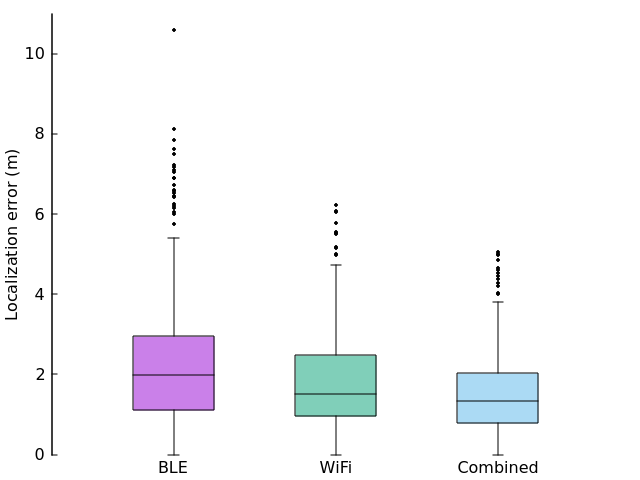
\includegraphics[width=0.5\textwidth]{img/wknn_errors_multiple}
		\par\end{centering}
	\caption{Comparison of localization accuracy for testing multiple fingerprints}
	\label{fig07c06}
\end{figure}

When comparing this figure with \fref{fig04c06} its shows decrease of median accuracy mainly for WiFi which also reflects on combined evaluation. Overall accuracy improved because errors are more clustered together and more evenly spread, there is also decrease of maximum error from 10 to 5.78 making it more viable in complex environments.

\subsection{Combining fingerprint data}\label{sec:CombiningFingerprintData}
Last evaluations did not prove tangible improvement of localization accuracy using wear technology in combination with mobile. For this reason next evaluation takes a different approach in combining data from multiple fingerprints based on device into one. Fingerprints are grouped based scan id, which identifies them being taken at the same place and time using different devices. Data of such fingerprints are combined into single one, reducing count of data for evaluation but hopefully increasing accuracy. Since there are multiple fingerprints combined the information about origin device is lost and there is no way to compare the technologies against each other.

There are two possible ways this will be implemented. First, copy all data into one fingerprint. Second, copy only BLE data and keep WiFi from phone, because it is known that wear WiFi precision is not sufficient and worsens the accuracy.

\begin{table}[h]
	\begin{center}
		\resizebox{\textwidth}{!}{
			\begin{tabular}{ l C{2cm} C{2cm} C{2cm} | C{2cm} C{2cm} C{2cm} }
				\cline{2-7}
				& \multicolumn{3}{c|}{WiFi with BLE} & \multicolumn{3}{c}{BLE only} \\
				\hline
				& BLE & WiFi & Combined & BLE & WiFi & Combined \\ 
				\hline	
				Mean & 2.12 & 0.93 & 0.88 & 2.12 & 0.88 & 0.83 \\
				Median & 1.73 & 0.87 & 0.86 & 1.73 & 0.80 & 0.83 \\
				Maximum & 13.99 & 7.19 & 6.99 & 13.99 & 8.00 & 7.04 \\
				\hline
			\end{tabular}
		}
		\caption{List of errors for fingerprint combination}
		\label{tab07c06}
	\end{center}
\end{table}

This approach as a whole seems to be big overall improvement in accuracy with a decrease when considering maximum error for BLE. Copying all data together improves precision compared to previous evaluation but it makes it only comparable to using mobile only. In numbers from \tref{tab05c06} mobile errors are 0.85m mean, 0.88m median and 6.06m maximum compared to 0.88m mean, 0.86m median and 6.99m maximum of this measurement. Improvement is only in median but other two values increase in comparison. 

Second approach of copying only BLE records to mobile fingerprints and keep its current WiFi precision while improving BLE proved to be finally better than only mobile precision. Comparing data from \tref{tab07c06} shows decrease of error for mean from 0.85 to 0.83 meters which is around 2.4\% and median from 0.88 to 0.83 meters reaching to 6\% improvement over mobile. One value that goes up is maximum error from 6.06 to 7.04 resulting in 16\% increase of this error.

\begin{figure}[h!]
	\begin{centering}
		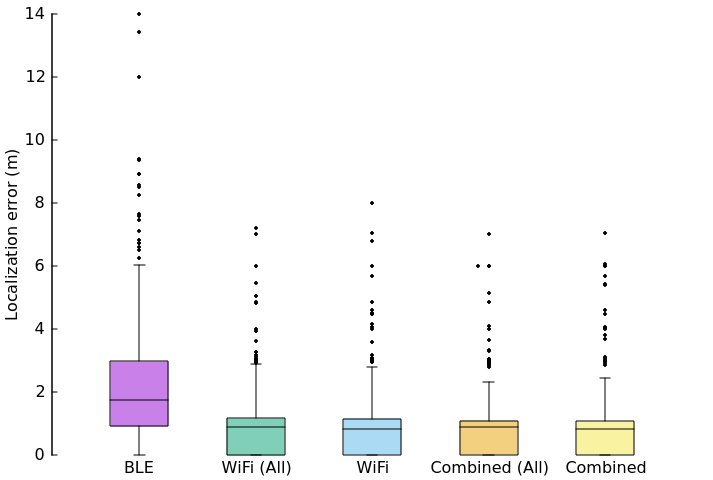
\includegraphics[width=0.6\textwidth]{img/wknn_errors_combined}
		\par\end{centering}
	\caption{Comparison of localization accuracy for combining fingerprints}
	\label{fig08c06}
\end{figure}

\fref{fig08c06} shows visualization of errors for both approaches. BLE errors are same for both cases and they seem to be somewhere between classic approach and testing of multiple fingerprints since it has more clustered values compared to classic one but not as multiple fingerprints testing. However, WiFi shows the best localization precision of all previous iterations. Both of these approaches seems to be comparable and each one has different merit to it, combination of all data seems to increase mean and median but lower down the maximum errors being more reliable in problematic places where the other one is the opposite.

\subsection{Map comparison}\label{sec:MapComparison}
To confirm previous results all errors were displayed on the map to compare them and also to find problematic spots of the evaluation. These maps contain only combined error of radio technologies to make it easier to read and not complicate it with differences between BLE and WiFi. There is also one other slight change to displayed result data where errors under 200 centimeters are set to display as a circle with such error which is mainly visible in the last image of \fref{fig09c06} because there are multiple fingerprints with 0 meters error.

\begin{figure}[h!]
	\begin{centering}
		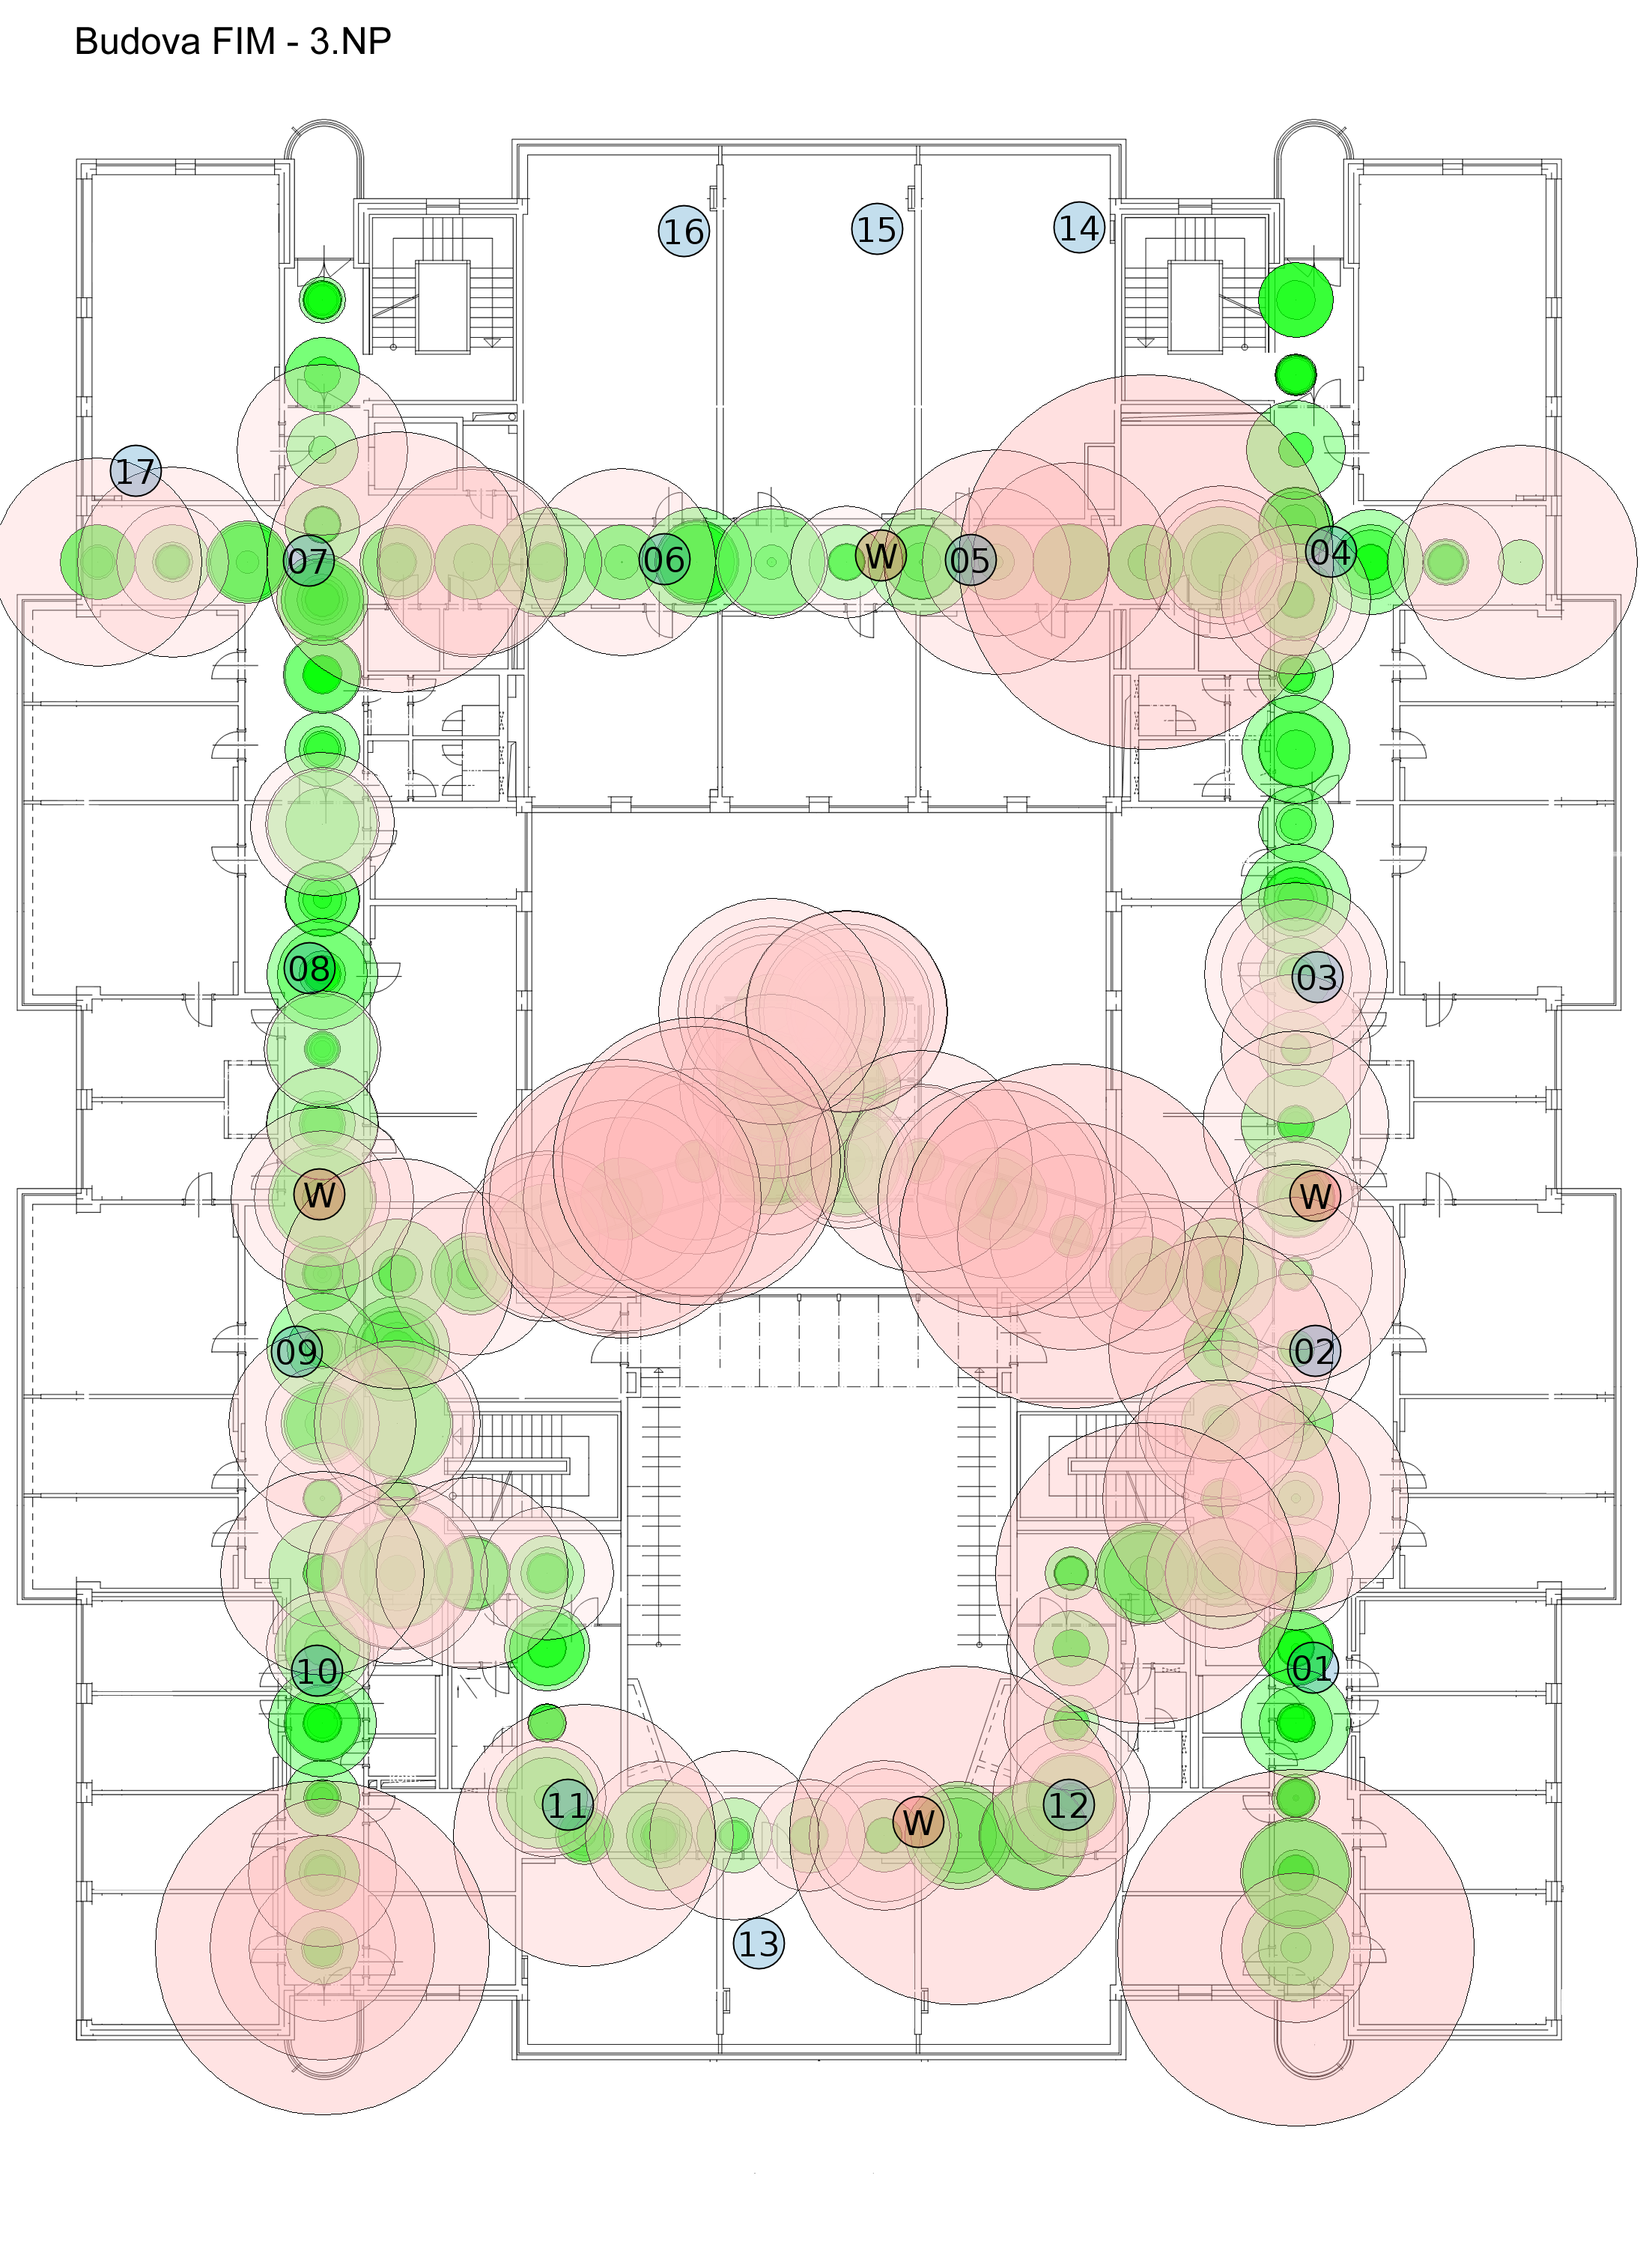
\includegraphics[width=0.4\textwidth]{img/combined_error_classic}
		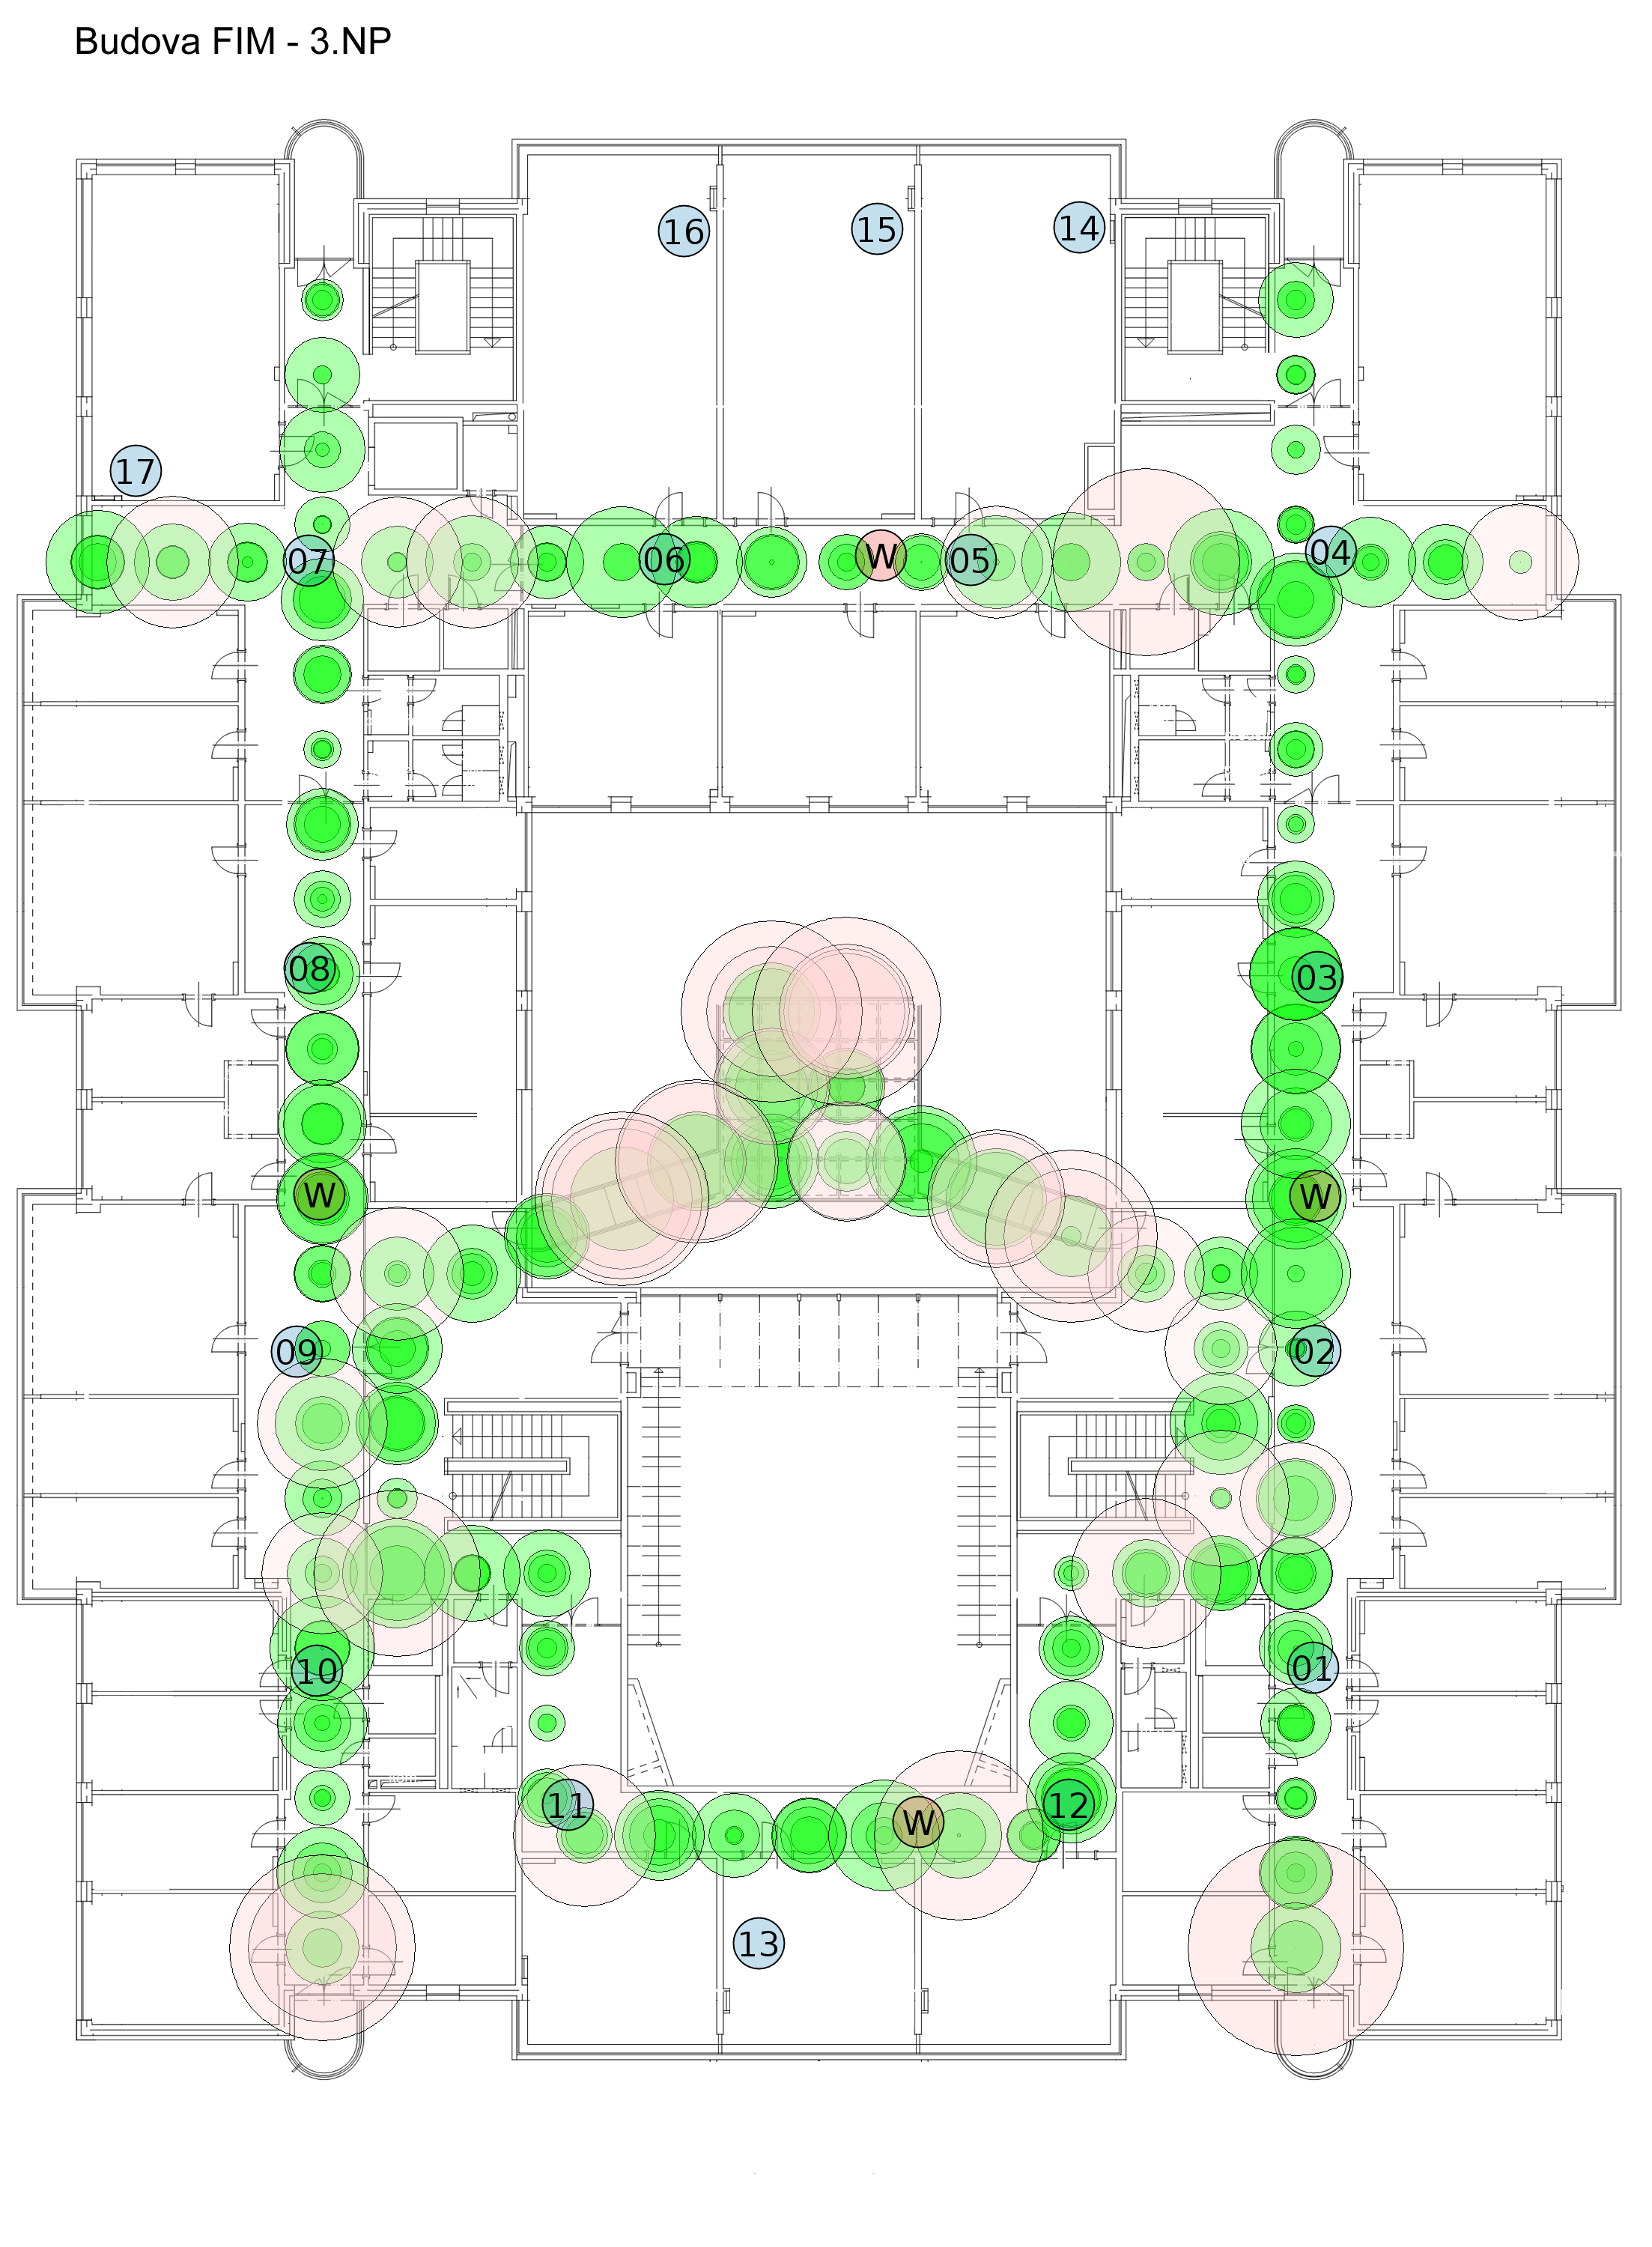
\includegraphics[width=0.4\textwidth]{img/combined_error_multiple_f}
		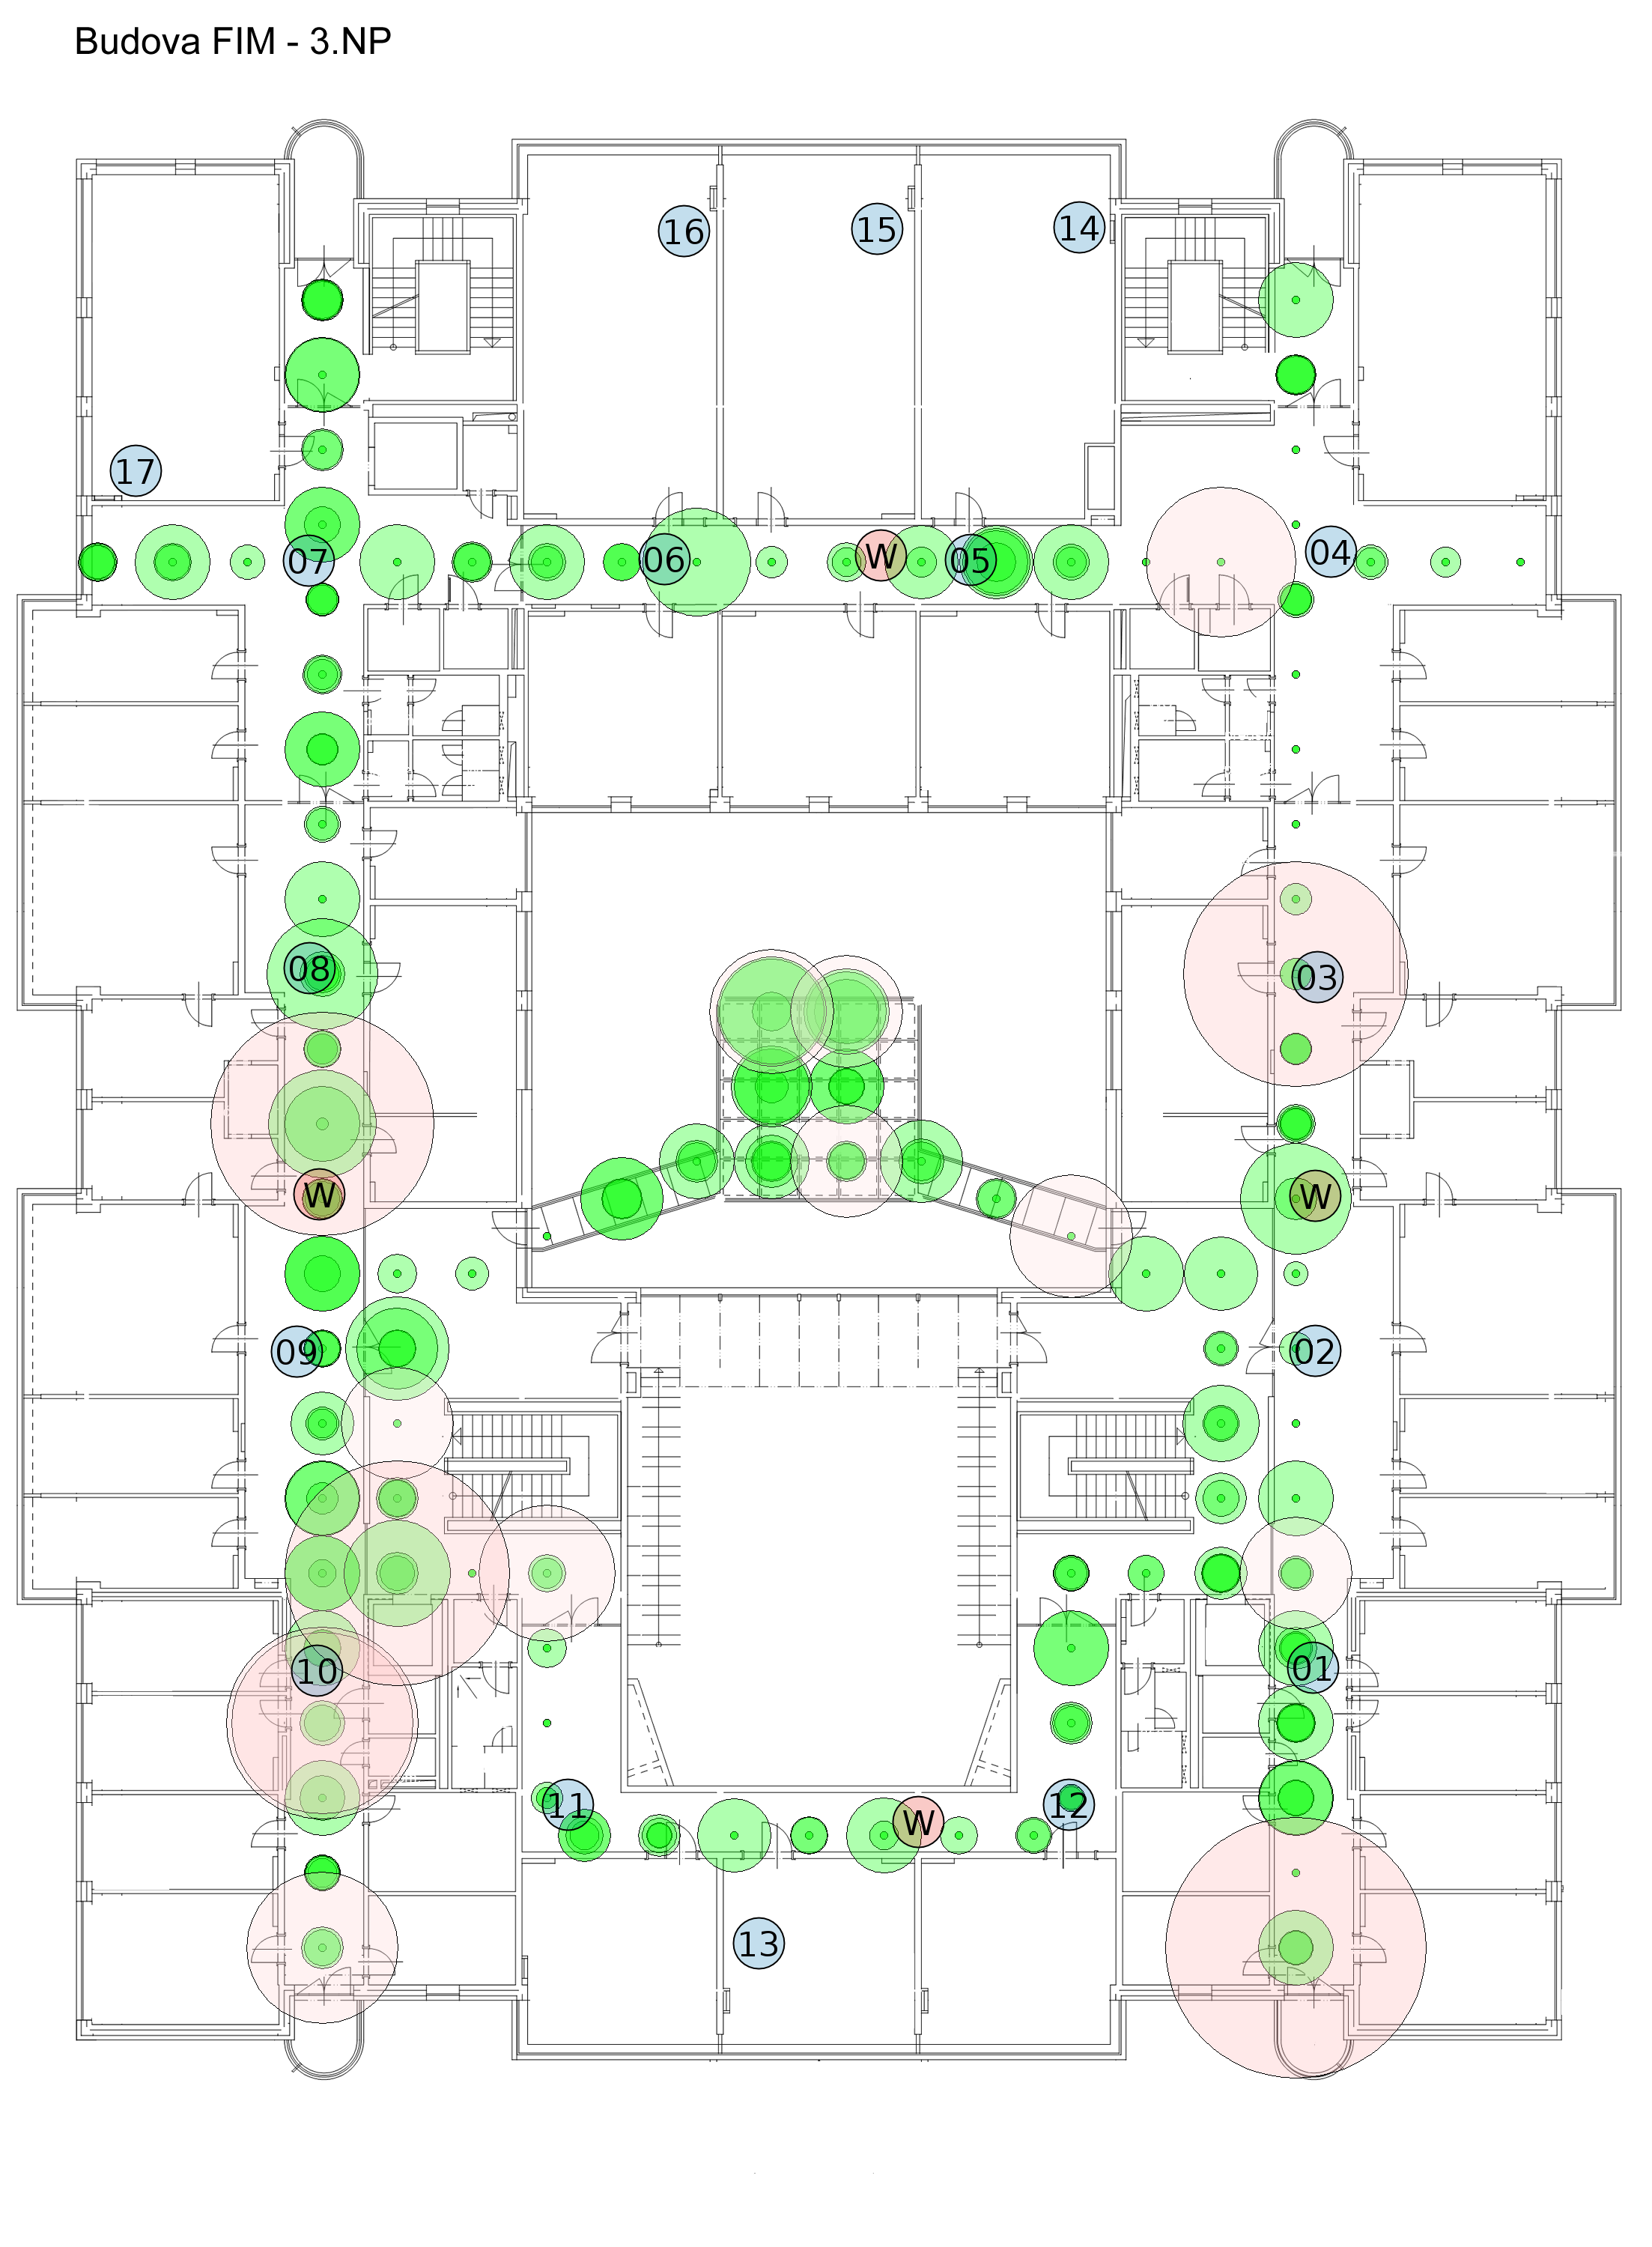
\includegraphics[width=0.4\textwidth]{img/combined_error_f_combination}
		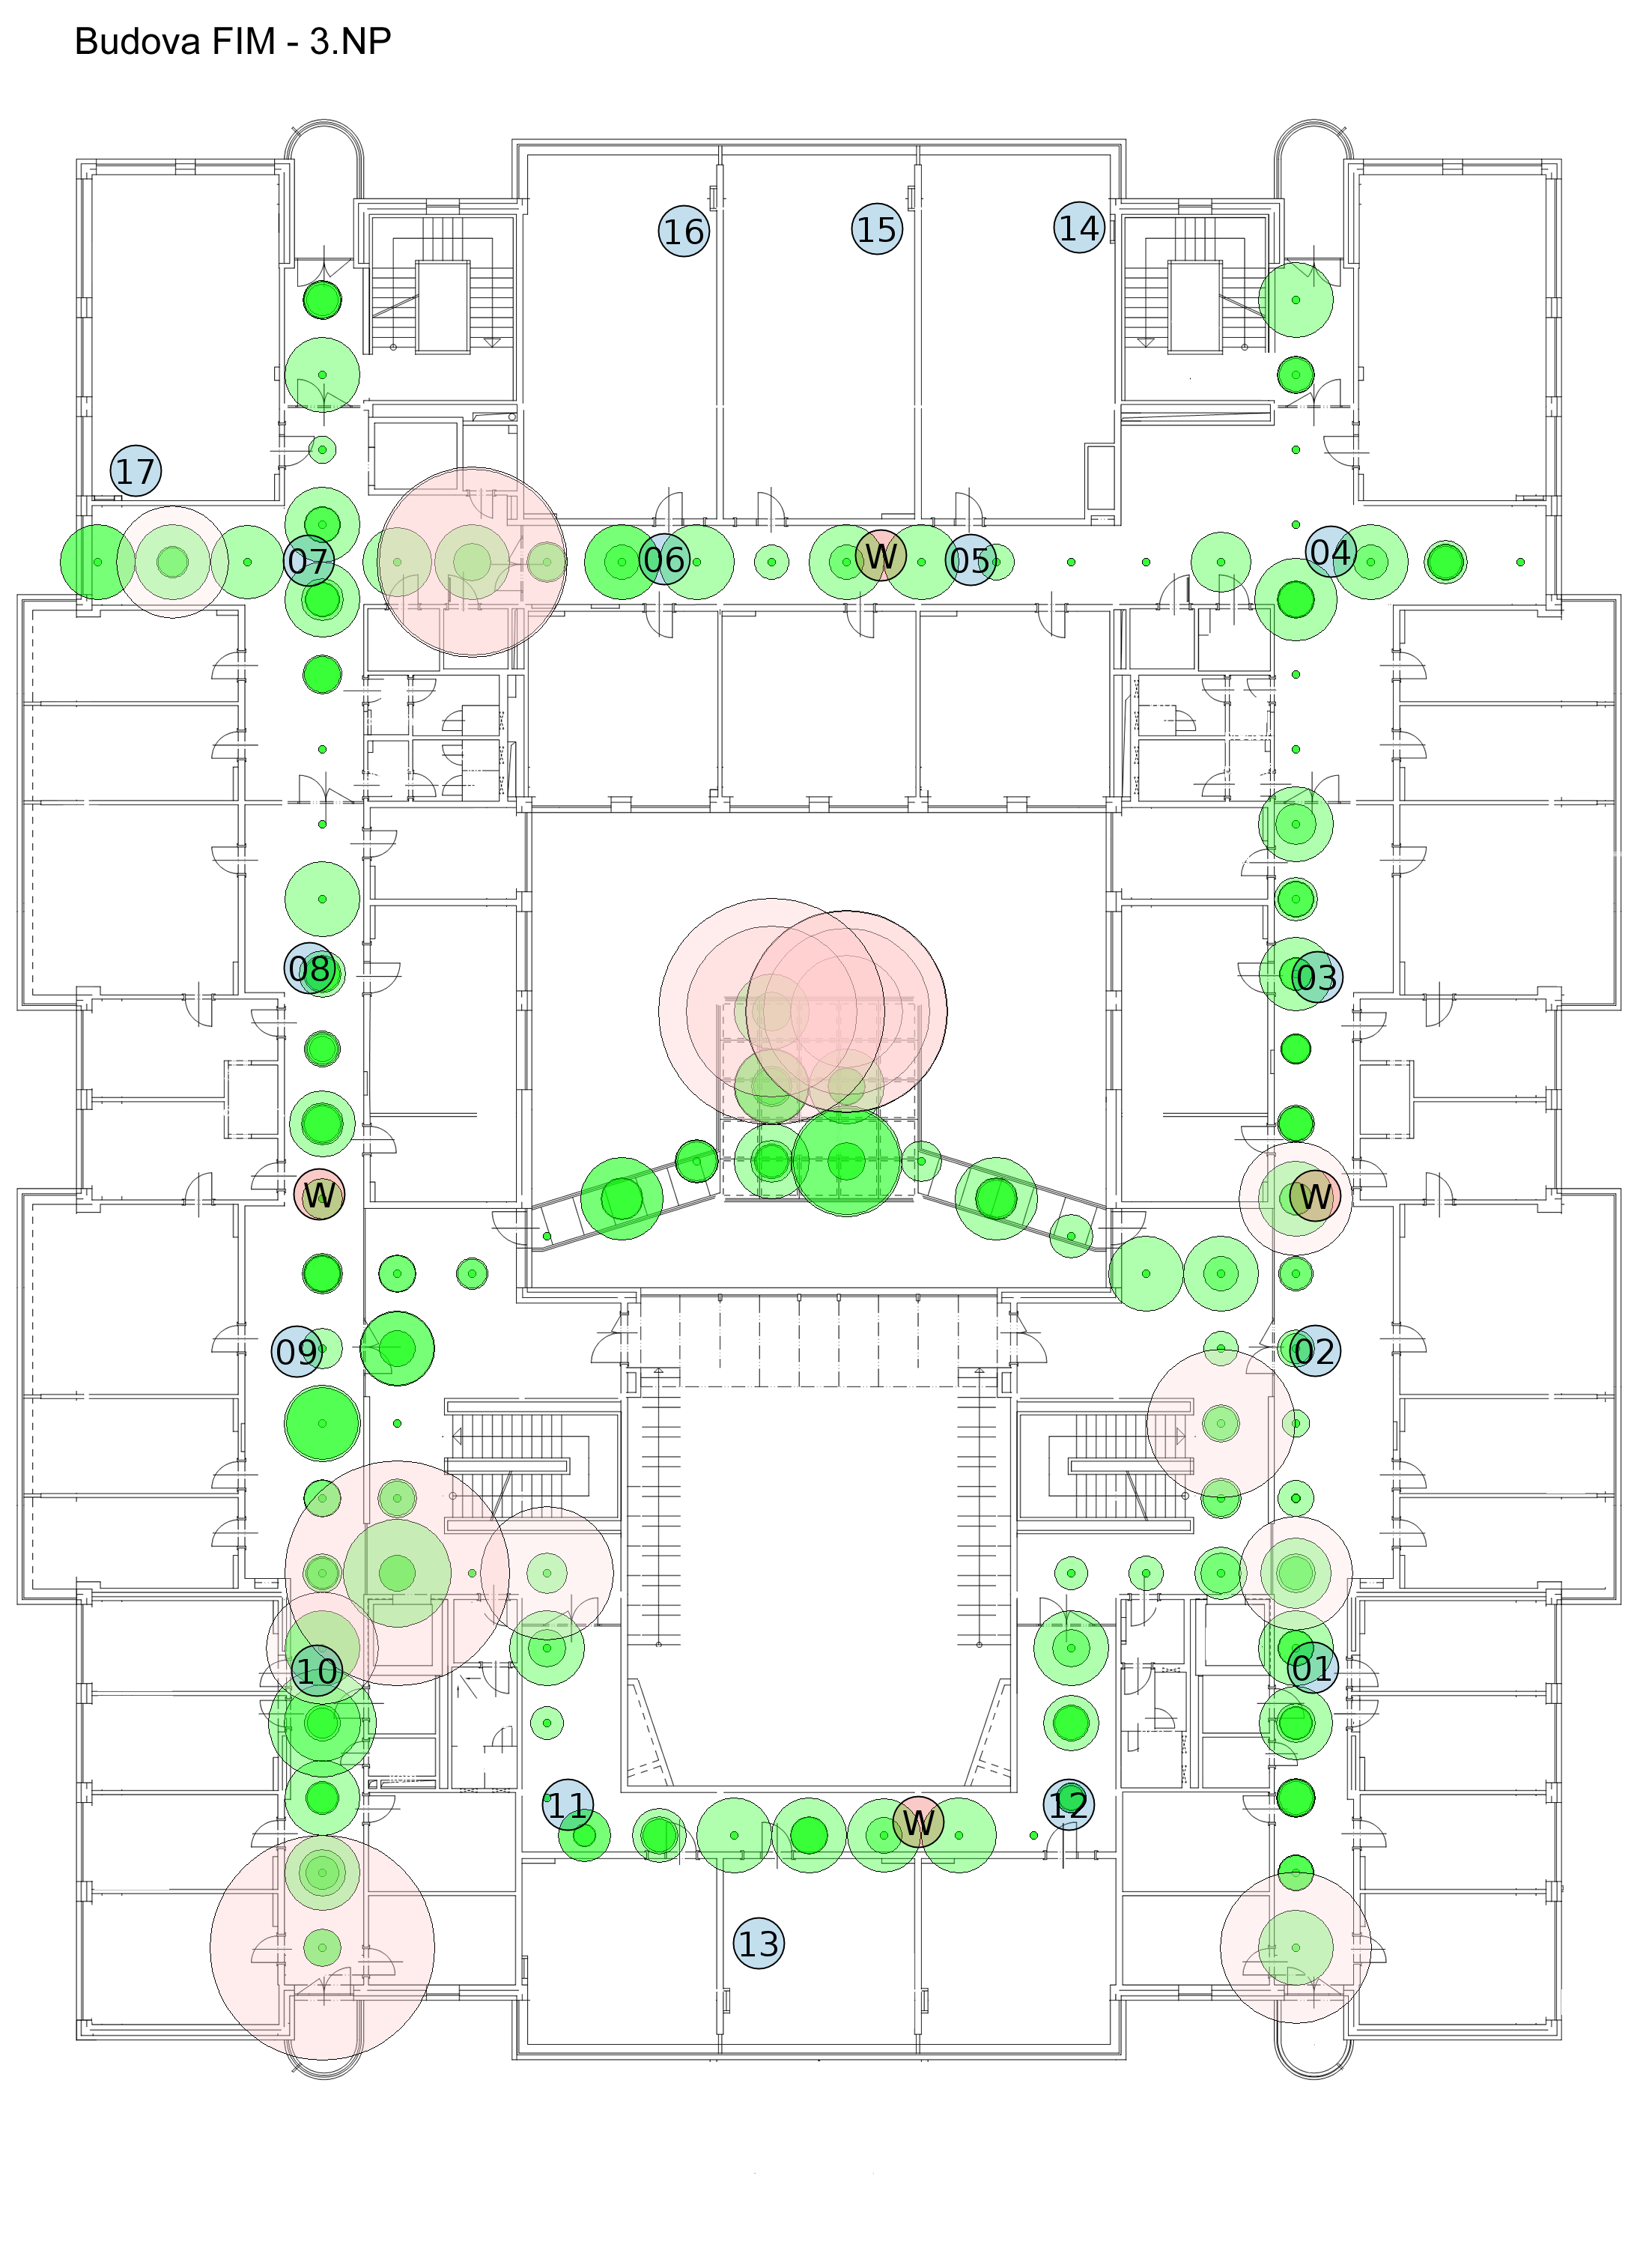
\includegraphics[width=0.4\textwidth]{img/phone_error}
		\par\end{centering}
	\caption{Maps of errors for all algorithms with last one for mobile error only}
	\label{fig09c06}
\end{figure}

\fref{fig09c06} shows map images for all previously described and evaluated algorithms and image with error only from mobile device. Top left image shows errors for classic evaluation ignoring device of origin. Top right is for next round of evaluation which takes two fingerprints with different device origin, calculates their position and averages it to improve accuracy. Bottom left picture is for the last evaluation which combines multiple fingerprints into one. Finally picture on the bottom right displays error just from phone device for a comparison with algorithm using data from wear.  

Classic evaluation shows a big amount of orange circles, which means that error of a specific fingerprint is over 3 meters, and most of them seem to be in the middle of Campus building where there are no beacons placed associated with this floor. The other problematic spots seems to be in the south part of the building (bottom part of the map). Rest of the places are not considered as problematic since they usually have only one fingerprint with error over 3 meters. There is 119 fingerprints with error higher than three which is around 14\%.

Moving to the second image, it shows a big improvement of the localization for all positions and filtering out which places may actually be problematic. Bringing count of fingerprints with high error from 119 to 35 which is just 4\%. As for final image, it illustrates the best precision of all algorithms with 82 fingerprints with 0 error and just 15 above 3 meters bringing it just under 2\%.